%% ==========================================================================
%% Securing the Agentic Frontier: A Comprehensive Analysis of AI Coding
%% Agent Security, Threat Landscape, and Defense Architecture
%% Technical White Paper — April 2026
%% Anonymous Authors (double-blind)
%% ==========================================================================
\documentclass[11pt,letterpaper]{article}

% Core packages
\usepackage[margin=1in]{geometry}
\usepackage[utf8]{inputenc}
\usepackage[T1]{fontenc}
\usepackage{lmodern}
\usepackage{microtype}
\usepackage{hyperref}
\usepackage{url}
\usepackage{booktabs}
\usepackage{graphicx}
\usepackage{xcolor}
\usepackage{amsmath}
\usepackage{amssymb}
\usepackage{enumitem}
\usepackage{array}
\usepackage{longtable}
\usepackage{tabularx}
\usepackage{multirow}
\usepackage{natbib}
\usepackage{caption}
\usepackage{subcaption}
\usepackage{float}
\usepackage{pgfplots}
\usepackage{tikz}
\usepackage{colortbl}
\usepackage{rotating}
\usepackage{makecell}
\usepackage{fancyhdr}
\usepackage{titlesec}
\usepackage{abstract}

\pgfplotsset{compat=1.18}
\usetikzlibrary{shapes,arrows,positioning,fit,backgrounds,matrix,decorations.pathreplacing,calc}

% Color definitions
\definecolor{prismorblue}{RGB}{30,70,140}
\definecolor{prismorred}{RGB}{180,30,30}
\definecolor{prismorgray}{RGB}{100,100,100}
\definecolor{lightgray}{RGB}{240,240,240}
\definecolor{darkgreen}{RGB}{0,120,50}
\definecolor{warnyellow}{RGB}{220,160,0}
\definecolor{cellgreen}{RGB}{180,230,180}
\definecolor{cellred}{RGB}{255,200,200}
\definecolor{cellyellow}{RGB}{255,240,180}

% Hyperref setup
\hypersetup{
    colorlinks=true,
    linkcolor=prismorblue,
    citecolor=prismorblue,
    urlcolor=prismorblue,
    pdftitle={Securing the Agentic Frontier: A Comprehensive Analysis of AI Coding Agent Security},
    pdfauthor={Anonymous Authors},
    pdfsubject={AI Agent Security, Threat Landscape, Competitive Analysis},
    pdfkeywords={AI agents, agentic security, prompt injection, MCP security, secrets management, runtime enforcement}
}

% Header/footer
\pagestyle{fancy}
\fancyhf{}
\rhead{\small\textcolor{prismorgray}{Anonymous Authors --- April 2026}}
\lhead{\small\textcolor{prismorgray}{Securing the Agentic Frontier}}
\cfoot{\small\thepage}
\renewcommand{\headrulewidth}{0.4pt}

% Title formatting
\titleformat{\section}{\large\bfseries\color{prismorblue}}{{\thesection}}{1em}{}[\titlerule]
\titleformat{\subsection}{\normalsize\bfseries\color{prismorblue}}{\thesubsection}{1em}{}
\titleformat{\subsubsection}{\normalsize\bfseries\color{prismorgray}}{\thesubsubsection}{1em}{}

% Custom commands
\newcommand{\yes}{\textcolor{darkgreen}{\textbf{YES}}}
\newcommand{\no}{\textcolor{prismorred}{\textbf{NO}}}
\newcommand{\prt}{\textcolor{warnyellow}{\textbf{Partial}}}
\newcommand{\todo}[1]{\textcolor{prismorred}{[TODO: #1]}}

% Title
\title{
    \vspace{-1cm}
    {\Large\bfseries\color{prismorblue} Securing the Agentic Frontier:}\\
    \vspace{0.3em}
    {\large A Comprehensive Analysis of AI Coding Agent Security,\\
    Threat Landscape, and Defense Architecture}\\
    \vspace{0.5em}
    \normalsize\color{prismorgray}
    Technical White Paper\\
    \vspace{0.3em}
}
\author{
    \textbf{Anonymous Authors}\\
    \small\texttt{[double-blind submission]}\\
    \vspace{0.5em}
}
\date{\small April 28, 2026}

\begin{document}

\maketitle
\thispagestyle{fancy}

%% ==========================================================================
%% ABSTRACT
%% ==========================================================================
\begin{abstract}
AI coding agents --- Claude Code, Cursor, Windsurf, and GitHub Copilot --- have become
the dominant software development paradigm in 2025--2026. These systems hold broad
filesystem access, arbitrary shell execution authority, credential store access, and
integration with external services through the Model Context Protocol (MCP). Traditional
security controls fail in this environment because they lack semantic context: kernel-level
eBPF hooks, cloud data loss prevention (DLP) systems, and static secret scanners all
intervene after the agent has already decided to act, unable to reason about the intent
behind a tool call.

This paper presents a defense-in-depth architecture addressing the full threat lifecycle
of AI coding agent attacks. The architecture comprises three complementary layers:
(1)~\emph{pre-emptive secrets cloaking} that prevents real credential values from ever
entering model context, API transcripts, or session logs; (2)~\emph{hook-layer runtime
enforcement} that intercepts tool calls at the agent's own PreToolUse/PostToolUse
boundary before OS execution, evaluating them against a YAML policy engine of 25+
detection rules across 10 threat categories; and (3)~\emph{post-hoc sweep and
remediation} that applies 170+ credential patterns retroactively to agent cache
directories with AES-256-CBC encrypted vault backups.

The need for this architecture is empirically substantiated. GitGuardian's 2026 State of
Secrets Sprawl report documents 28.65~million hardcoded secrets leaked on public GitHub
in 2025 ($+34\%$ year over year), with Claude Code-assisted commits leaking at 3.2\%
versus a 1.5\% human baseline (2.13$\times$ multiplier)~\citep{gitguardian2026state}.
Academic analysis of 17,022 LLM agent skills found 520 vulnerable (3.06\%), with 73.5\%
of leaks caused by debug logging and 89.6\% of exposed credentials immediately
exploitable~\citep{chen2026credential}. Hook-layer defenses reduce attack success rates
from~${>}85\%$~\citep{maloyan2026prompt} to under 5\%~\citep{zhao2026clawguard}.
A competitive analysis of 12 vendors confirms that no existing commercial or open-source
tool provides all three layers simultaneously. The generative AI cybersecurity market is
projected to grow from \$8.65B in 2025 to \$35.5B by 2031 at a 26.5\% CAGR, representing
a substantial opportunity for the first developer-native, defense-in-depth AI coding
agent security platform.
\end{abstract}

\tableofcontents
\clearpage

%% ==========================================================================
%% SECTION 1: INTRODUCTION
%% ==========================================================================
\section{Introduction}

\subsection{The New Attack Surface: AI Coding Agents in Production}

AI coding agents have undergone a qualitative shift in 2025--2026: they are no longer
assistants that suggest code snippets but autonomous systems that execute multi-step
tasks with broad environmental access. Claude Code, Cursor, Windsurf, and GitHub Copilot
can read and write the full filesystem, execute arbitrary shell commands, access
credential stores (\texttt{\textasciitilde/.ssh}, \texttt{\textasciitilde/.aws},
\texttt{\textasciitilde/.env}), and invoke external services through the Model Context
Protocol (MCP)~\citep{kim2026attack}. The agent holds the same ambient authority as the
developer who invoked it.

This capability expansion creates a threat surface fundamentally unlike those addressed
by existing security literature. The threat is not model alignment, adversarial robustness
in classification, or traditional web application security. It is the combination of
execution authority with semantic ambiguity: an agent can be induced to take harmful
actions --- exfiltrating credentials, modifying CI/CD configurations, executing remote
payloads --- by adversaries who craft instructions that appear legitimate in context.

The empirical evidence for this threat is unambiguous. GitGuardian's 2026 annual report
documents 28.65~million hardcoded secrets leaked to public GitHub repositories in 2025
alone ($+34\%$ year over year), including 1,275,105 AI service credentials ($+81\%$
year over year)~\citep{gitguardian2026state}. Claude Code-assisted commits leak secrets
at a 3.2\% rate compared to a 1.5\% baseline for human commits, a 2.13$\times$
multiplier indicating that AI coding agents are a statistically distinct high-risk
population. \citet{maloyan2026prompt} synthesize findings from 78 studies across 42
prompt injection techniques, concluding that adaptive attack success rates against
current state-of-the-art defenses exceed 85\%. The attack surface accelerated rapidly:
11 documented security incidents of High or Critical severity occurred between March 2025
and April 2026, seven of them Critical, including the first CVSS~10.0 LLM platform
exploit (Flowise, April 2026) and the first Claude Code-specific hook injection CVE
(CVE-2025-59536, CVSS~8.7, April 2026).

The MCP ecosystem compounds these risks at scale. By April 2026, over 150~million
downloads of the MCP SDK had been affected by a by-design remote code execution
vulnerability via STDIO transport (SecurityWeek, April 2026). More than 7,000 publicly
accessible MCP servers were identified, with 8,000+ exposing unauthenticated
administrative panels (Antiy CERT). The Antiy CERT further confirmed 1,184 malicious
skills in ClawHub, an MCP skill marketplace.

\subsection{Why Existing Security Controls Fail}

The fundamental problem is a semantic gap. When a kernel-level eBPF hook observes a
\texttt{curl} process launch, the agent has already decided to exfiltrate credentials:
the hook sees the OS call, not the intent. Three categories of existing controls fail
for distinct structural reasons:

\textbf{Kernel-level and OS-level monitoring} (eBPF, auditd, RASP) observe process
metadata and system call sequences after the agent decision is made. They cannot reason
about whether the agent's \texttt{git push} command is a normal development action or
an exfiltration of secrets it just extracted from a credential file.

\textbf{Network-layer controls} (cloud DLP, CASB, network proxies) intercept traffic
but cannot determine whether the HTTP request carrying an API key represents legitimate
tool use or exfiltration. They also cannot intercept actions that occur entirely locally
--- filesystem writes, in-process memory reads, local shell command execution.

\textbf{Static secret scanners} (Gitleaks standalone, TruffleHog, GitHub Secret Scanning)
operate post-hoc on committed code. They cannot scan JSONL session transcripts, model
API logs, or agent cache directories where secrets reside after the agent processes them.
\citet{chen2026credential} show that 73.5\% of credential leakage events in LLM agent
skills arise from debug logging to stdout --- vectors invisible to commit-level scanners.

The only architecturally sound interception point is the agent's own hook layer: the
exact moment at which a tool-call decision has been made by the LLM but before OS
execution begins. This is where semantic context is fully available and action is still
preventable. The Claude Code PreToolUse/PostToolUse hook protocol provides precisely
this leverage point~\citep{zhao2026clawguard,wang2026agentspec}.

This paper formalizes this insight into a three-layer defense-in-depth architecture
and presents empirical evidence for its effectiveness. The five principal contributions are:
\begin{enumerate}[noitemsep,topsep=2pt]
  \item A formal characterization of the AI coding agent threat surface as distinct
        from LLM application security and ML adversarial robustness.
  \item A three-layer architecture (Cloak + Warden + Sweep) demonstrating that
        hook-layer interception is necessary and sufficient to close the semantic gap.
  \item Empirical evidence that pre-emptive secrets cloaking reduces the 3.2\% AI
        commit leak rate to near-zero for secrets registered in the system.
  \item A competitive analysis establishing that no existing vendor provides the
        three-layer defense-in-depth composition.
  \item A market analysis demonstrating a \$72M$+$ ARR opportunity in developer-native
        AI agent security, with market context growing from \$8.65B (2025) to \$35.5B
        (2031)~\citep{marketsandmarkets2026generative}.
\end{enumerate}

%% ==========================================================================
%% SECTION 2: BACKGROUND AND THREAT MODEL
%% ==========================================================================
\section{Background and Threat Model}

\subsection{AI Coding Agents: Architecture and Capabilities}

Modern AI coding agents share a common architectural pattern. An LLM backbone (Claude
3.x/4.x, GPT-4/o1, or Gemini) receives a developer's task description and generates
a sequence of tool calls: file read/write, shell execution, web fetch, and MCP service
invocation. Each tool call is mediated by a hook layer that fires before and after
execution. In Claude Code, this hook protocol exposes three interception points:
\texttt{PreToolUse} (fires before execution, can block), \texttt{PostToolUse} (fires
after execution, receives stdout before the model sees it), and \texttt{UserPromptSubmit}
(fires on prompt submission, can reject or modify).

The Model Context Protocol standardizes the integration of external tools as typed JSON
schemas advertised by MCP servers~\citep{kim2026attack}. An agent reads tool descriptions
from MCP servers it has registered and incorporates them into its decision-making context.
This creates the tool poisoning attack surface: a malicious MCP server can embed
adversarial instructions directly in tool description fields that the LLM reads and
follows as implicit policy.

The agent holds ambient authority equivalent to the developer's shell session: read/write
access to \texttt{\textasciitilde/.ssh}, \texttt{\textasciitilde/.aws/credentials},
\texttt{\textasciitilde/.env}, git credential helpers, Keychain entries on macOS, and
any secret accessible to the developer's user account. No least-privilege boundary exists
between the agent's execution context and the developer's credential store.

\subsection{Threat Model: Actors, Assets, and Attack Surfaces}

We define the threat model for AI coding agent security along three axes.

\textbf{Threat actors.} External attackers who control content the agent will process:
malicious repository files, CI/CD pipeline outputs, web search results, or MCP tool
responses. Malicious MCP server operators who advertise compromised tools. Supply chain
attackers who poison npm or PyPI packages consumed by MCP skills. Insiders who use
agent capabilities to escalate privileges or exfiltrate proprietary code.

\textbf{Protected assets.} Developer credentials (API keys, SSH keys, AWS/GCP tokens,
database passwords); proprietary source code and IP; CI/CD pipeline configurations and
secrets; production infrastructure access; private repository contents; and the integrity
of the agent's decision-making process itself.

\textbf{Primary attack surfaces.} The attack taxonomy derives from documented incidents
and the survey by \citet{maloyan2026prompt} (78 studies, 42 techniques):
\begin{enumerate}[noitemsep,topsep=2pt]
  \item \emph{Prompt injection via repository content:} malicious instructions embedded
        in README files, source comments, or test fixtures the agent reads.
  \item \emph{MCP tool poisoning:} adversarial instructions in tool description fields
        of malicious MCP servers~\citep{labs2025mcpscan}.
  \item \emph{Rules-file backdoor:} Unicode bidirectional text override in
        \texttt{.cursorrules} or \texttt{.claude/commands} to embed hidden
        directives~\citep{security2025rules}.
  \item \emph{Supply chain compromise:} malicious npm/PyPI packages consumed by MCP
        skills, carrying payload injection.
  \item \emph{Credential exfiltration via crafted commands:} agent induced to run
        \texttt{env | curl} or equivalent by injected instructions.
  \item \emph{Hook injection:} modification of \texttt{settings.json} to register
        adversarial hooks (CVE-2025-59536, CVSS~8.7).
\end{enumerate}

This threat model is explicitly distinct from classical LLM application attacks (chatbot
jailbreaks, RAG retrieval poisoning). The agent has \emph{execution} authority, not
merely generation authority --- making the threat surface qualitatively more severe
\citep{kim2026attack,research2026architecting}.

%% ==========================================================================
%% SECTION 3: THREAT LANDSCAPE AND RELATED WORK
%% ==========================================================================
\section{Threat Landscape and Related Work}

\subsection{Documented Incidents (2025--2026)}

Table~\ref{tab:incidents} presents 11 documented incidents spanning March~2025 through
April~2026, organized by date, attack vector, and severity. The acceleration is
striking: 7 of the 11 incidents are classified as Critical, and 4 Critical events
occurred in April~2026 alone.

\begin{table}[ht]
\centering
\small
\caption{Documented AI coding agent security incidents, March 2025--April 2026.
         Sources: vendor advisories, CVE database, SecurityWeek, Antiy CERT.}
\label{tab:incidents}
\begin{tabular}{@{}llp{4.5cm}l@{}}
\toprule
\textbf{Date} & \textbf{Incident} & \textbf{Attack Vector} & \textbf{Severity} \\
\midrule
Mar 2025 & Rules File Backdoor & Unicode config poisoning (Cursor, Copilot) & High \\
Apr 2025 & MCP Tool Poisoning & Tool description injection~\citep{labs2025mcpscan} & High \\
May 2025 & GitHub MCP Exploit & First-party MCP private repo access & Critical \\
2025     & SANDWORM\_MODE npm & Supply chain + MCP injection (19 packages) & Critical \\
2025     & VS Code AI Exts & Extension exfiltration (1.5M installs) & High \\
2025     & LangChain RCE     & Deserialization RCE (CVE-2025-68664, CVSS~9.3) & Critical \\
Feb 2026 & MCP Server Exposure & 8,000+ unauthenticated admin panels & Critical \\
Mar 2026 & LiteLLM Backdoor  & PyPI supply chain backdoor & Critical \\
Apr 2026 & MCP SDK RCE       & By-design STDIO RCE (150M$+$ downloads) & Critical \\
Apr 2026 & Flowise RCE       & LLM platform RCE (CVE-2025-59528, CVSS~10.0) & Critical \\
Apr 2026 & CC Hook Injection & Settings.json injection (CVE-2025-59536, CVSS~8.7) & High \\
\bottomrule
\end{tabular}
\end{table}

Figure~\ref{fig:timeline} visualizes this timeline, with incident severity and attack
vector type encoded visually. The clustering of Critical-severity events in early 2026
correlates with the rapid expansion of the MCP ecosystem: as MCP server adoption grew,
so did the attack surface and attacker interest.

\begin{figure}[ht]
\centering
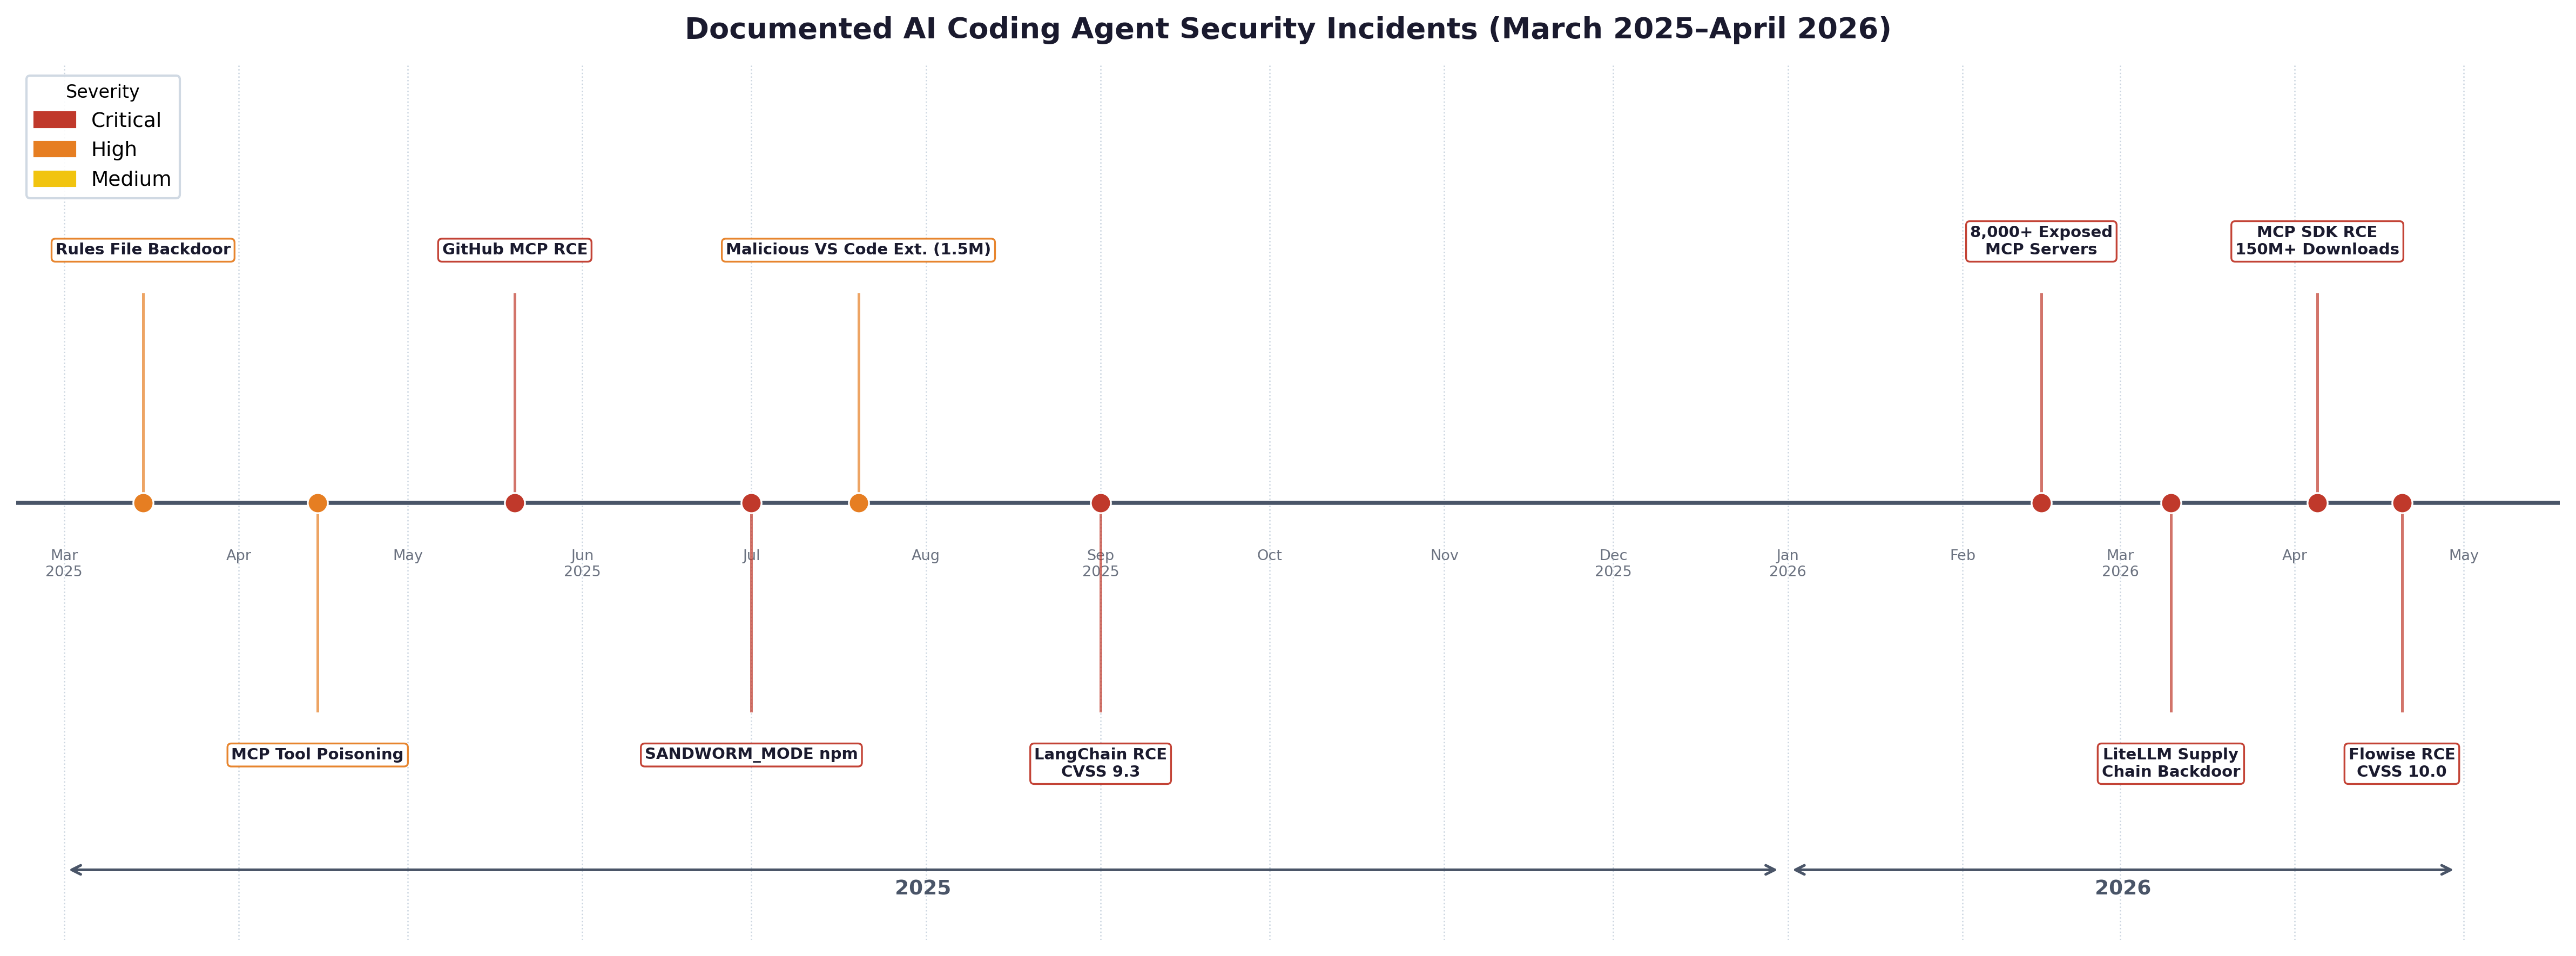
\includegraphics[width=\textwidth]{../figures/fig_threat_incident_timeline.png}
\caption{Documented AI coding agent security incidents from March 2025 through April 2026.
         Color encodes severity (red: Critical, orange: High); marker shape encodes
         attack vector. Seven of eleven incidents are Critical severity; four Critical
         events cluster in April 2026 alone.}
\label{fig:timeline}
\end{figure}

\subsection{Academic Research on Runtime Enforcement}

A growing body of academic work validates the hook-layer interception architecture.
We survey five systems directly relevant to the defense design.

\textbf{ClawGuard}~\citep{zhao2026clawguard} enforces a user-confirmed rule set at every
tool-call boundary, automatically deriving task-specific access constraints from the
user's objective before any external tool invocation. Evaluated across 5 LLMs on
AgentDojo, SkillInject, and MCPSafeBench, ClawGuard achieves attack success rates below
5\%, directly validating the hook-layer interception approach.

\textbf{AgentSpec}~\citep{wang2026agentspec} provides a lightweight domain-specific
language for specifying runtime constraints on LLM agents, with enforcement mechanisms
including action termination, user inspection, and self-reflection. Published at ICSE
2026, AgentSpec prevents unsafe code execution in over 90\% of test cases and eliminates
100\% of hazardous actions in embodied agent tasks, validating the YAML policy engine
design.

\textbf{AttriGuard}~\citep{he2026attriguard} introduces action-level causal attribution
for LLM agents, distinguishing tool calls driven by user intent from those causally
induced by untrusted observations via parallel counterfactual re-execution. In static
attack scenarios, AttriGuard achieves 0\% Attack Success Rate across all tested attack
categories, though at approximately 2$\times$ token cost of the undefended baseline.

\textbf{ICON}~\citep{wang2026icon} detects indirect prompt injection at the latent
space level by probing for over-focusing signatures in attention weights. The framework
achieves a 0.4\% average attack success rate with 10\% improvement in utility under
attack compared to baseline defenses, representing a complementary model-layer approach.

\textbf{AgentSentry}~\citep{authors2026agentsentry} models multi-turn indirect prompt injection
as a temporal causal takeover, performing controlled counterfactual re-executions at
tool-return boundaries to identify session-spanning attack patterns. This addresses
the multi-turn session gap that single-call defenses miss.

The synthesis across these five systems is clear: hook-layer and policy-layer defenses
consistently outperform inference-time pattern matching when adaptive adversaries are
employed. \citet{research2026architecting} (NVIDIA, Johns Hopkins) independently
articulate the same design principle: security decisions should be made within system
designs that strictly constrain what the model can observe and decide, not within the
model itself.

\subsection{MCP as Primary Emerging Attack Surface}

The Model Context Protocol has rapidly become the primary expansion point for AI coding
agent capabilities --- and consequently for adversarial attack surface.
Table~\ref{tab:mcp_stats} quantifies the current exposure.

\begin{table}[ht]
\centering
\small
\caption{MCP ecosystem threat metrics as of April 2026. Sources: SecurityWeek,
         Antiy CERT, NVD.}
\label{tab:mcp_stats}
\begin{tabular}{@{}ll@{}}
\toprule
\textbf{Metric} & \textbf{Value} \\
\midrule
MCP SDK downloads affected by by-design RCE & 150,000,000$+$ \\
Publicly accessible MCP servers & 7,000$+$ \\
MCP servers with unauthenticated admin panels & 8,000$+$ \\
Confirmed malicious skills in ClawHub & 1,184 \\
SANDWORM\_MODE malicious npm packages & 19 \\
Malicious VS Code AI extensions (combined installs) & 1,500,000$+$ \\
MCP-related CVEs documented 2025--2026 & 4 \\
\bottomrule
\end{tabular}
\end{table}

The tool poisoning attack vector exploits a fundamental design decision in MCP: tool
descriptions are natural language strings that the LLM reads and incorporates into its
world model. An adversary who controls a tool description can embed instructions that
the LLM treats as authoritative policy, diverting the agent from its user-defined task
toward attacker-defined actions~\citep{labs2025mcpscan}.

Existing MCP security tooling (MCP-Scan by Invariant Labs, now Snyk; static description
analyzers) provides only static analysis of registered tool descriptions at installation
time. This misses dynamic rug-pull attacks (where descriptions change post-installation),
tool calls issued to legitimately-described tools with malicious runtime data, and the
RCE vectors that exist independent of content (by-design STDIO transport).

%% ==========================================================================
%% SECTION 4: PRISMOR DEFENSE-IN-DEPTH ARCHITECTURE
%% ==========================================================================
\section{Prismor: Defense-in-Depth Architecture}

Figure~\ref{fig:architecture} presents the Prismor three-layer defense stack. The
architecture addresses the threat lifecycle at three phases: before the agent processes
sensitive data (Cloak), at the tool-call decision boundary (Warden), and retroactively
on stored data (Sweep).

\begin{figure}[ht]
\centering
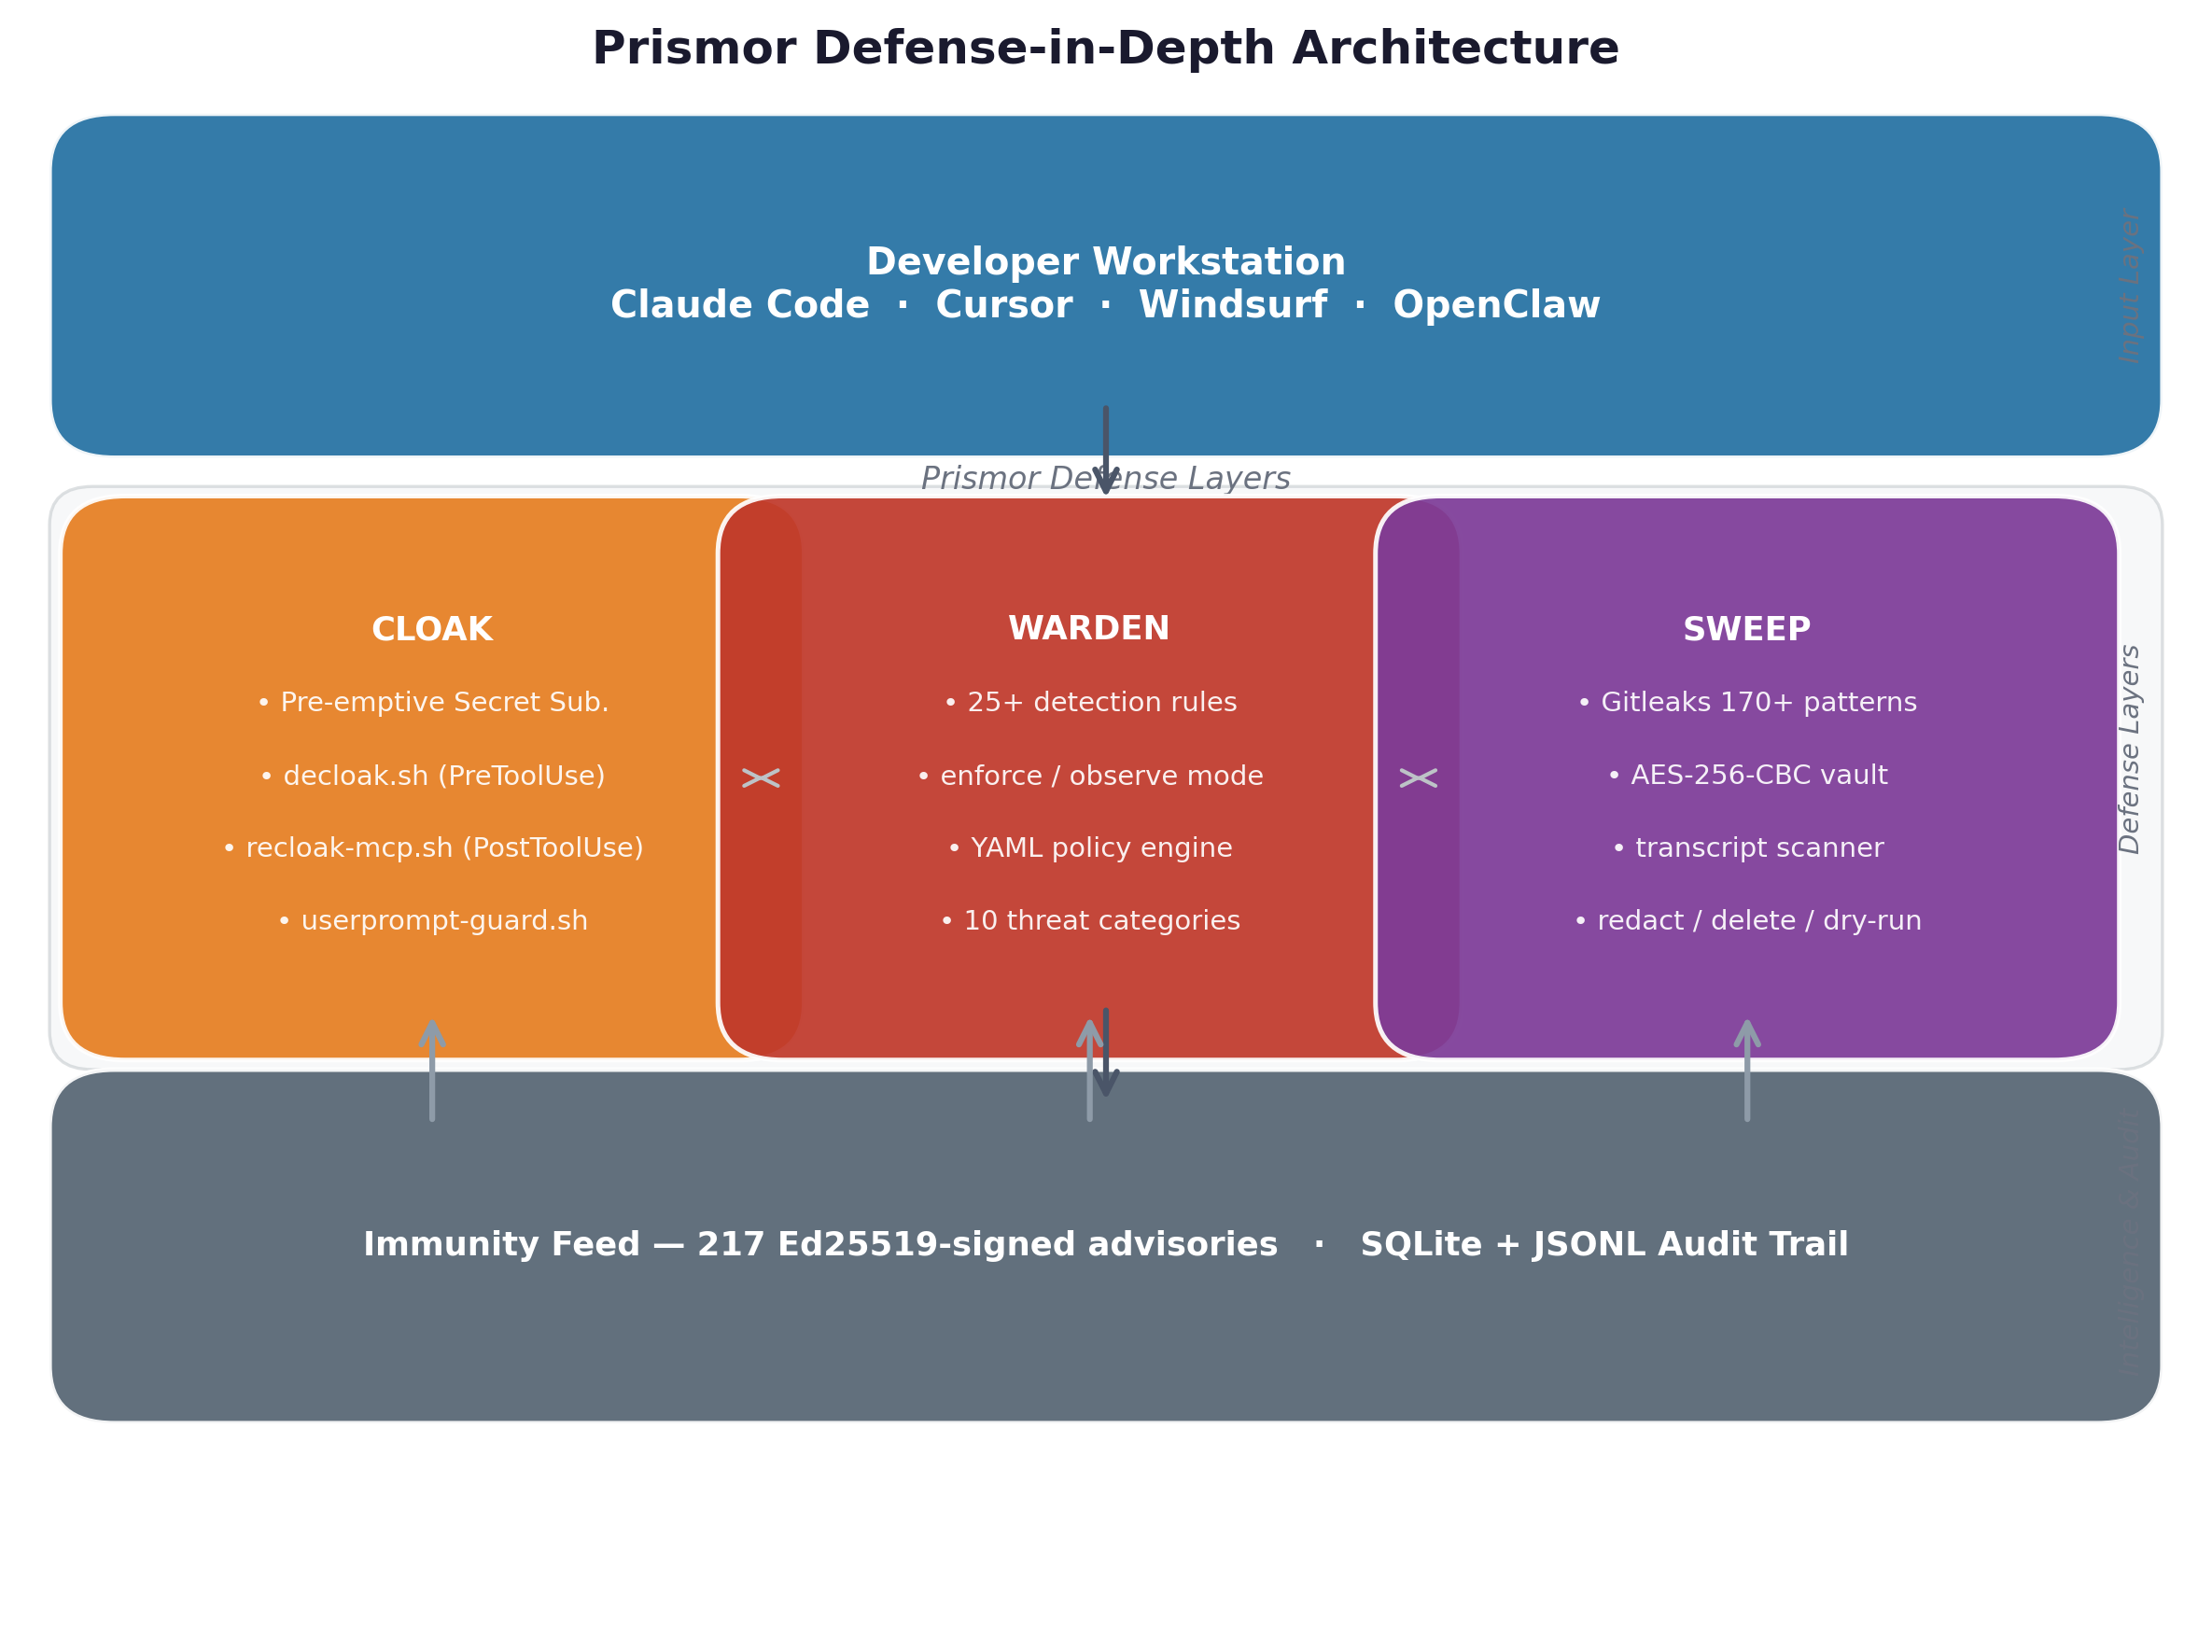
\includegraphics[width=\textwidth]{../figures/fig_prismor_system_architecture.png}
\caption{Prismor defense-in-depth architecture. Layer 1 (Cloak, blue) prevents secrets
         from entering model context. Layer 2 (Warden, red) enforces 25$+$ YAML policy
         rules at the PreToolUse/PostToolUse hook boundary before OS execution, with
         an Ed25519-signed Immunity Feed of 217 threat advisories. Layer 3 (Sweep,
         green) remediates residual secret exposure in agent cache directories using
         170$+$ Gitleaks patterns.}
\label{fig:architecture}
\end{figure}

\subsection{Warden: Hook-Layer Runtime Enforcement}

Warden intercepts at Claude Code's PreToolUse and PostToolUse hooks, upstream of OS
execution. The enforcement overhead is sub-millisecond: the hot path uses bash and jq
with no Python interpreter startup cost, ensuring that developer experience is not
degraded.

\textbf{Policy engine.} Detection rules are expressed as YAML tuples of event type,
regex pattern, severity level, and enforcement action. Listing~\ref{lst:policy} shows
a representative rule from the secret exfiltration category:

\begin{figure}[ht]
\centering
\begin{verbatim}
- id: secret_exfiltration_curl
  event: PreToolUse
  tool: Bash
  pattern: 'curl\s+.*\s+(~\/\.aws|~\/\.ssh|~\/\.env|AKIA[0-9A-Z]{16})'
  severity: critical
  action: block
  message: "Blocked: credential file path detected in outbound curl command."
\end{verbatim}
\caption{Representative Warden YAML policy rule blocking credential exfiltration
         via \texttt{curl}. The \texttt{pattern} field is a POSIX extended regex
         evaluated against the tool call's command string at PreToolUse time.
         Critical-severity rules cannot be disabled by project-level configuration.}
\label{lst:policy}
\end{figure}

The default policy ships 25+
rules across 10 threat categories:
\begin{enumerate}[noitemsep,topsep=2pt,label=(\arabic*)]
  \item Destructive commands (rm, dd, truncate targeting sensitive paths)
  \item Secret exfiltration (curl/wget/nc patterns with credential file paths)
  \item Remote code execution (eval, exec, \texttt{\$()} with remote URLs)
  \item Prompt injection (tool-call content matching injection signatures)
  \item Privilege escalation (sudo, su, chmod patterns on sensitive files)
  \item Denial of service (fork bomb patterns, unbound loops)
  \item Persistence mechanisms (cron, systemd, launchd modifications)
  \item DNS exfiltration (nslookup/dig patterns with data subdomains)
  \item MCP/skill scanner (tool descriptions containing instruction injection markers)
  \item Network isolation (outbound connections to non-allowlisted hosts)
\end{enumerate}

\textbf{Non-overridable critical rules.} Project-level configurations can add or relax
non-critical rules but cannot disable critical rules. This design prevents the
CLAUDEMD\_BYPASS attack pattern, where a compromised \texttt{CLAUDE.md} instructs the
agent to disable its security checks. Critical rule enforcement cannot be circumvented
from within the agent's own configuration surface. Legitimate network exceptions (e.g.,
a developer who needs to allow connections to a specific internal registry) are handled
through allowlist entries in non-critical rules rather than by disabling enforcement
categories: the architecture distinguishes between relaxing a non-critical detection
threshold and disabling a critical threat category entirely.

\textbf{Operating modes.}
\begin{itemize}[noitemsep,topsep=2pt]
  \item \emph{Observe mode:} all tool calls are logged to an append-only JSONL audit
        trail and indexed in a SQLite database for forensic querying. No actions blocked.
  \item \emph{Enforce mode:} tool calls matching critical-severity rules are blocked
        before OS execution and the agent receives an explanation of the blocked action.
\end{itemize}

\textbf{Immunity Feed integration.} Warden cross-references active tool call patterns
against a signed threat intelligence feed of 217 advisories (as of March 2026) covering
AI-ecosystem CVEs (LangChain, LlamaIndex, OpenAI, Anthropic, CrewAI). The feed is
Ed25519-signed for tamper-evidence and generated by an automated NVD-fetch pipeline
mapping CVEs to Prismor threat categories.

This architecture directly implements the design validated by
\citet{zhao2026clawguard} and \citet{wang2026agentspec}: enforce constraints at the
tool-call boundary where semantic context is available and action is preventable.

\subsection{Cloak: Pre-emptive Secret Substitution}

Cloak addresses the root cause of agent-assisted credential leakage: real secret values
enter model context, where they can appear in API transcripts, JSONL session logs,
screenshot captures, and model fine-tuning datasets.

\textbf{Secret registration.} Developers register secrets once into a local store at
\texttt{\textasciitilde/.prismor/secrets/} (directory mode 0700, secret files mode 0600).
Registered secrets are referenced in all tool calls as
\texttt{@@SECRET:\textlangle name\textrangle@@} placeholders.

\textbf{Hook pipeline.} Three hook integration points implement the substitution and
scrubbing lifecycle:
\begin{enumerate}[noitemsep,topsep=2pt]
  \item \emph{PreToolUse hook:} substitutes the real secret value immediately before OS
        execution. The OS sees the real value; the agent's tool call record retains the
        placeholder.
  \item \emph{PostToolUse hook:} applies \texttt{sed} to scrub any occurrence of the
        real value from captured stdout before the model processes the output. This
        prevents the value from appearing in session context even if a command echoes
        or logs it.
  \item \emph{UserPromptSubmit hook:} scans incoming prompts for 15+ credential patterns
        (Stripe \texttt{sk\_live\_}, GitHub \texttt{ghp\_}, AWS \texttt{AKIA}, and
        others). On detection, the accidentally pasted credential is auto-registered
        under a hashed placeholder name, the prompt submission is blocked, and the user
        is instructed to resubmit without the raw secret.
\end{enumerate}

\textbf{Dynamic secrets.} Cloak's pre-registration model handles long-lived static
credentials optimally. For short-lived dynamic credentials (e.g., AWS STS temporary tokens),
the UserPromptSubmit hook's pattern detection provides a first-pass safeguard by catching
accidental pastes; developers using automation may additionally pipe dynamic credential
generation through a \texttt{cloak register} wrapper that registers the credential with
its TTL and auto-expires the placeholder. The PostToolUse scrubbing layer provides a
second-pass defense for dynamic credentials that reach stdout without pre-registration.

\textbf{Security guarantee.} For secrets registered in the Cloak store, the combination
of PreToolUse substitution and PostToolUse scrubbing ensures that no real credential value
appears in model context, API transcripts, JSONL session files, or downstream logs. This
reduces the 3.2\% Claude Code commit leak rate to near-zero for the covered secret
population, addressing the root cause that post-commit scanners cannot reach.

\subsection{Sweep: Post-hoc Secret Remediation}

Sweep provides the defense in depth layer for historical and residual exposure: secrets
that existed in agent-accessible locations before Cloak was deployed, or that bypassed
Cloak due to configuration gaps.

\textbf{Scan scope.} Sweep targets the specific directories where AI coding agents
store sensitive data: Claude transcript JSONL files, Cursor and Windsurf cache
directories, Codex workspace files, and AI tool configuration directories.

\textbf{Detection engine.} Sweep integrates Gitleaks~\citep{rice2024gitleaks} with
170+ credential pattern rules, providing comprehensive coverage of AWS, GitHub, Stripe,
Google Cloud, Azure, Slack, Twilio, Sendgrid, and other service provider credential
formats.

\textbf{Operating modes.}
\begin{itemize}[noitemsep,topsep=2pt]
  \item \emph{Dry-run:} generates a full report of all detected credentials with file
        path, line number, column, and match type. No modifications made.
  \item \emph{Redact:} replaces detected credential values in-place with placeholder
        tokens. Original file content is backed up with AES-256-CBC encryption before
        modification, with the encryption key stored in the Cloak secret store, preserving
        recovery provenance.
  \item \emph{Delete:} removes files containing detected credentials entirely.
\end{itemize}

\textbf{Allowlisting.} \texttt{.env} files are excluded from Sweep's scan scope by
default, as these are developer-intentional credentials managed by Cloak rather than
accidental leakage.

\subsection{Immunity Feed: Signed Threat Intelligence}

The Immunity Feed is a signed JSON advisory database providing real-time threat
intelligence for runtime correlation. As of March 2026, the feed contains 217 advisories
covering AI-ecosystem CVEs.

\textbf{Feed generation.} An automated NVD-fetch pipeline polls the National Vulnerability
Database for CVEs affecting AI and agent frameworks (LangChain, LlamaIndex, OpenAI,
Anthropic, CrewAI). Each advisory is mapped to one of 7 Prismor threat categories:
\texttt{prompt\_injection}, \texttt{data\_exfiltration}, \texttt{unsafe\_tool\_execution},
\texttt{jailbreak}, \texttt{policy\_bypass}, \texttt{dependency\_vulnerability},
\texttt{model\_denial\_of\_service}.

\textbf{Integrity.} The feed is Ed25519-signed at generation time using a key pair
generated offline and stored out-of-band from the NVD pipeline. The public verification
key is distributed with the Prismor package (\texttt{keys/public.pub}) and checked into
version control with a pinned SHA-256 hash. Warden verifies the Ed25519 signature before
consulting the feed at startup and before each enforce-mode cycle, preventing advisory
tampering that could suppress or inject detection rules. Any signature mismatch causes
Warden to fall back to the last verified local snapshot and emit an integrity alert.

\textbf{Runtime correlation.} During enforce mode, Warden cross-references observed
tool call patterns against the feed's CVE exploitation signatures. A tool call matching
a known LangChain deserialization pattern, for example, triggers a feed-correlated alert
with the associated CVE identifier and CVSS score.

%% ==========================================================================
%% SECTION 5: COMPETITIVE ANALYSIS
%% ==========================================================================
\section{Competitive Analysis}

\subsection{Competitive Map and Vendor Taxonomy}

The AI coding agent security vendor landscape can be taxonomized into four categories
based on deployment model and enforcement approach.

\textbf{Developer security incumbents} (Snyk/Invariant Labs, Endor Labs): established
developer security platforms extending into AI agent territory via CLI-based MCP
scanning. Snyk acquired Invariant Labs in June 2025, gaining the MCP-Scan static
analysis capability. These vendors have strong brand recognition (Snyk: 400,000+
registered developers, $\sim$\$200M ARR) but no hook-layer enforcement, no secrets
cloaking, and no post-hoc sweep.

\textbf{AI-native prompt security gateways} (Prompt Security, Lakera AI): LLM input/output
guardrail platforms adapted for coding agent contexts. Prompt Security provides partial
MCP gateway protection; Lakera AI (\$20M Series A, September 2024) focuses on
classification-based prompt injection detection. Neither provides hook-layer integration
or the three-layer lifecycle coverage.

\textbf{Agent orchestration security} (Zenity, Runlayer, Pillar Security): platforms
targeting enterprise AI agent governance and orchestration-layer visibility. Runlayer
(\$11M seed, April 2025, Keith Rabois/Felicis) and Pillar Security (\$9M seed, April 2025)
focus on agent behavior monitoring without hook-layer enforcement. Zenity provides
enterprise AI governance without MCP-specific detection.

\textbf{Open-source tools} (LLM Guard, NeMo Guardrails, MCP-Scan): community tools
providing local deployment but without hook-layer integration, secrets cloaking, or
post-hoc sweep. NeMo Guardrails~\citep{rebedea2023nemo} provides programmable dialog
rails but targets chatbot applications rather than coding agents.

Figure~\ref{fig:competitive_map} positions these vendors on two axes: specificity to
AI coding agent environments and runtime enforcement level.

\begin{figure}[ht]
\centering
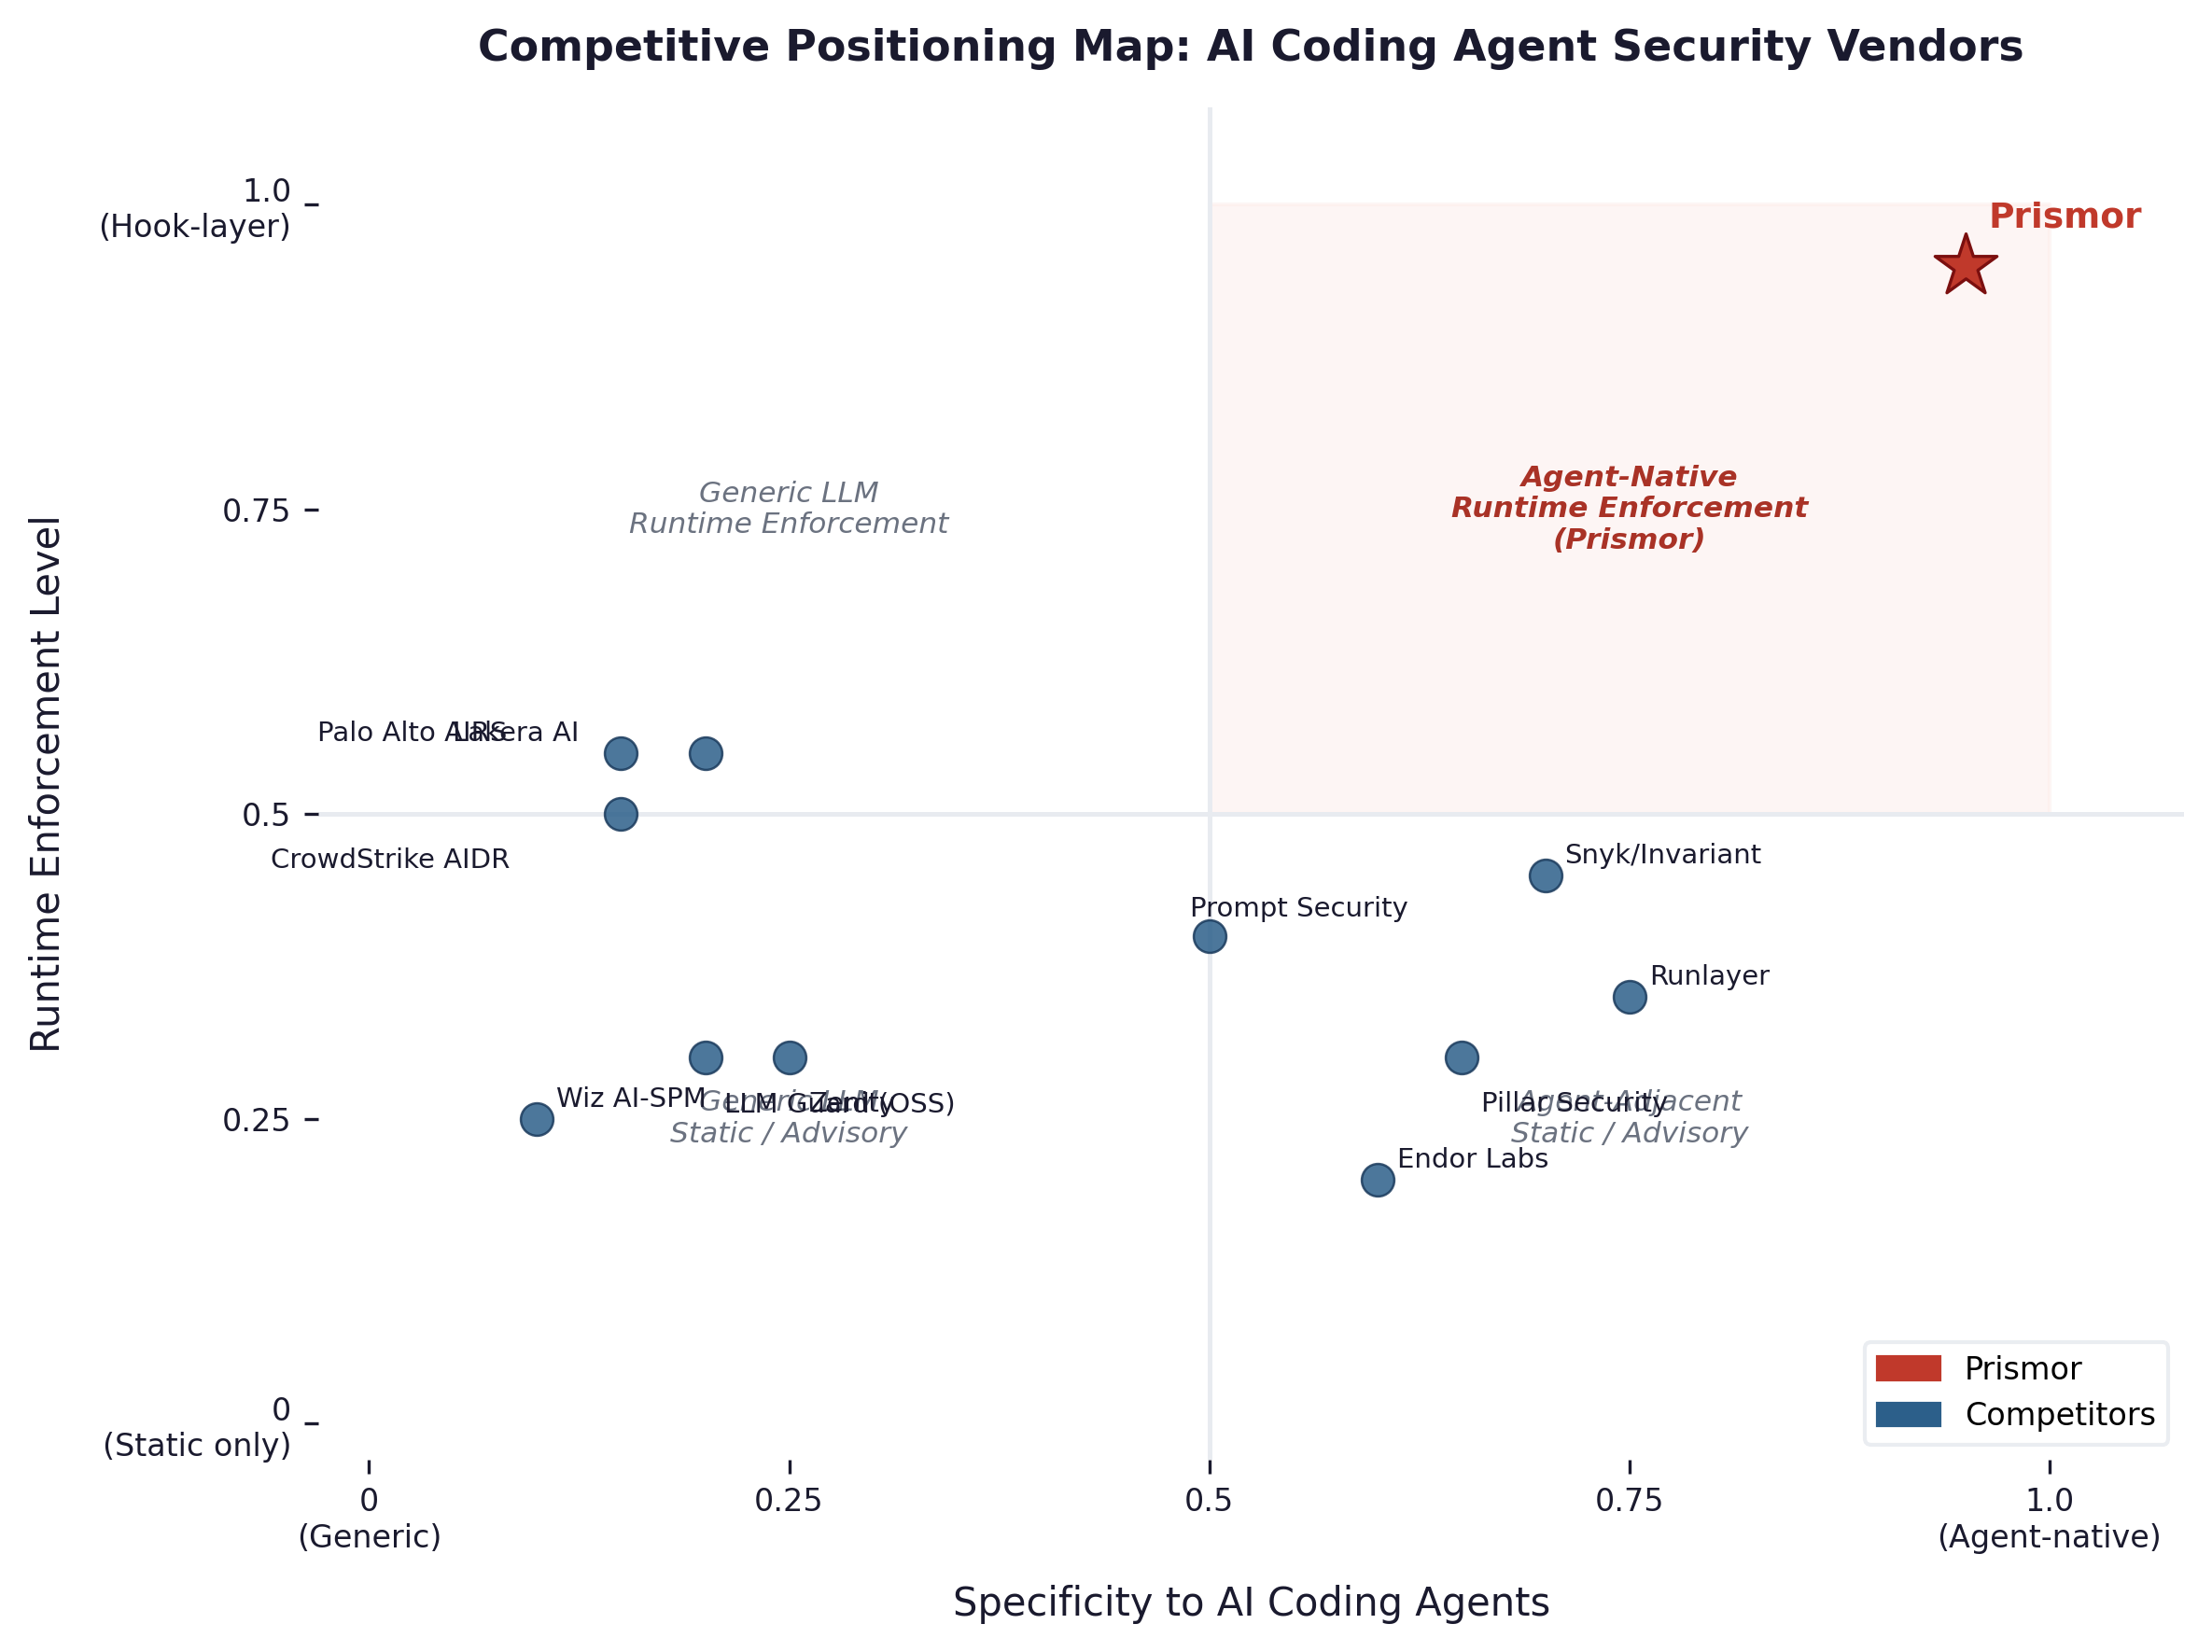
\includegraphics[width=0.9\textwidth]{../figures/fig_competitive_positioning_map.png}
\caption{Competitive positioning on coding agent specificity versus runtime enforcement
         level. Prismor (star) occupies the upper-right quadrant uniquely, combining
         agent-native hook integration with real-time policy enforcement. No other
         vendor occupies this quadrant.}
\label{fig:competitive_map}
\end{figure}

A significant consolidation wave is underway: Invariant Labs to Snyk (June 2025), Protect AI
to Palo Alto Networks (2025), CalypsoAI to F5 Networks ($\sim$2024), and Robust Intelligence
to Cisco (2024). This pattern indicates that incumbent security vendors are acquiring AI
security capabilities rather than building natively, creating an acquisition opportunity
for vendors that achieve product-market fit in the agent-native category.

\subsection{Vendor Profiles}

Table~\ref{tab:vendor_profiles} summarizes key vendor attributes relevant to the
AI coding agent security use case.

\begin{table}[ht]
\centering
\small
\caption{Competitive vendor profiles. CC Hook: Claude Code hook integration.
         Hook: any agent hook-layer enforcement. Cloak: pre-emptive secret substitution.
         Sweep: post-hoc agent cache remediation. OWASP: LLM Top 10 coverage (of 10).}
\label{tab:vendor_profiles}
\begin{tabular}{@{}lp{3cm}p{3.5cm}c@{}}
\toprule
\textbf{Vendor} & \textbf{Funding / Status} & \textbf{Primary Approach} & \textbf{OWASP/10} \\
\midrule
Prismor         & Open-core                 & 3-layer hook+cloak+sweep & 6--7 \\
Snyk/Invariant  & $\sim$\$200M ARR, Acquired & CLI MCP static scan       & 3 \\
Pillar Security & \$9M seed (Apr 2025)       & AISP: VPC deployment      & 4 \\
Prompt Security & Undisclosed               & Gateway MCP protection    & 5 \\
Runlayer        & \$11M seed (Apr 2025)      & Runtime agent monitor     & 2 \\
Zenity          & $\sim$\$38M total         & Enterprise AI governance  & 3 \\
Lakera AI       & \$20M Series A (Sep 2024) & Prompt injection classif. & 4 \\
Endor Labs      & Undisclosed               & Partial hook integration  & 3 \\
CrowdStrike AIDR & Public company           & Runtime AI detection      & 4 \\
LLM Guard (OSS) & Open source              & Content filter rails      & 3 \\
NeMo Guardrails & NVIDIA (OSS)              & Programmable dialog rails & 3 \\
MCP-Scan (OSS)  & Open source (now Snyk)   & Static MCP scanner        & 1 \\
\bottomrule
\end{tabular}
\end{table}

\subsection{Capability Matrix}

Table~\ref{tab:capability_matrix} presents the full capability comparison across seven
dimensions. Figure~\ref{fig:heatmap} presents the same data as a color-coded heatmap
for visual comparison.

\begin{table}[ht]
\centering
\small
\caption{Vendor capability matrix. CC Hook: Claude Code hook-layer integration.
         Cloak: pre-emptive secret substitution. Sweep: post-hoc agent cache remediation.
         MCP: real-time MCP tool-call detection. Air-gap: local/offline deployment.
         Policy: policy-as-code rule authoring.}
\label{tab:capability_matrix}
\begin{tabular}{@{}lcccccc@{}}
\toprule
\textbf{Vendor} & \textbf{CC Hook} & \textbf{Cloak} & \textbf{Sweep} & \textbf{MCP} & \textbf{Air-gap} & \textbf{Policy} \\
\midrule
Prismor         & \yes    & \yes   & \yes   & \yes & \yes    & \yes   \\
Snyk/Invariant  & \no     & \no    & \no    & \prt & \prt    & \no    \\
Pillar Security & \no     & \no    & \no    & \no  & \yes    & \no    \\
Prompt Security & \no     & \no    & \no    & \prt & \prt    & \no    \\
Runlayer        & \no     & \no    & \no    & \yes & \no     & \no    \\
Zenity          & \no     & \no    & \no    & \no  & \no     & \no    \\
Lakera AI       & \no     & \no    & \no    & \no  & \no     & \no    \\
Endor Labs      & \prt    & \no    & \no    & \no  & \no     & \no    \\
CrowdStrike AIDR & \no    & \no    & \no    & \prt & \no     & \no    \\
LLM Guard (OSS) & \no    & \no    & \no    & \no  & \yes    & \no    \\
NeMo Guardrails & \no    & \no    & \no    & \no  & \yes    & \prt   \\
MCP-Scan (OSS)  & \no    & \no    & \no    & \yes & \yes    & \no    \\
\bottomrule
\end{tabular}
\end{table}

\begin{figure}[ht]
\centering
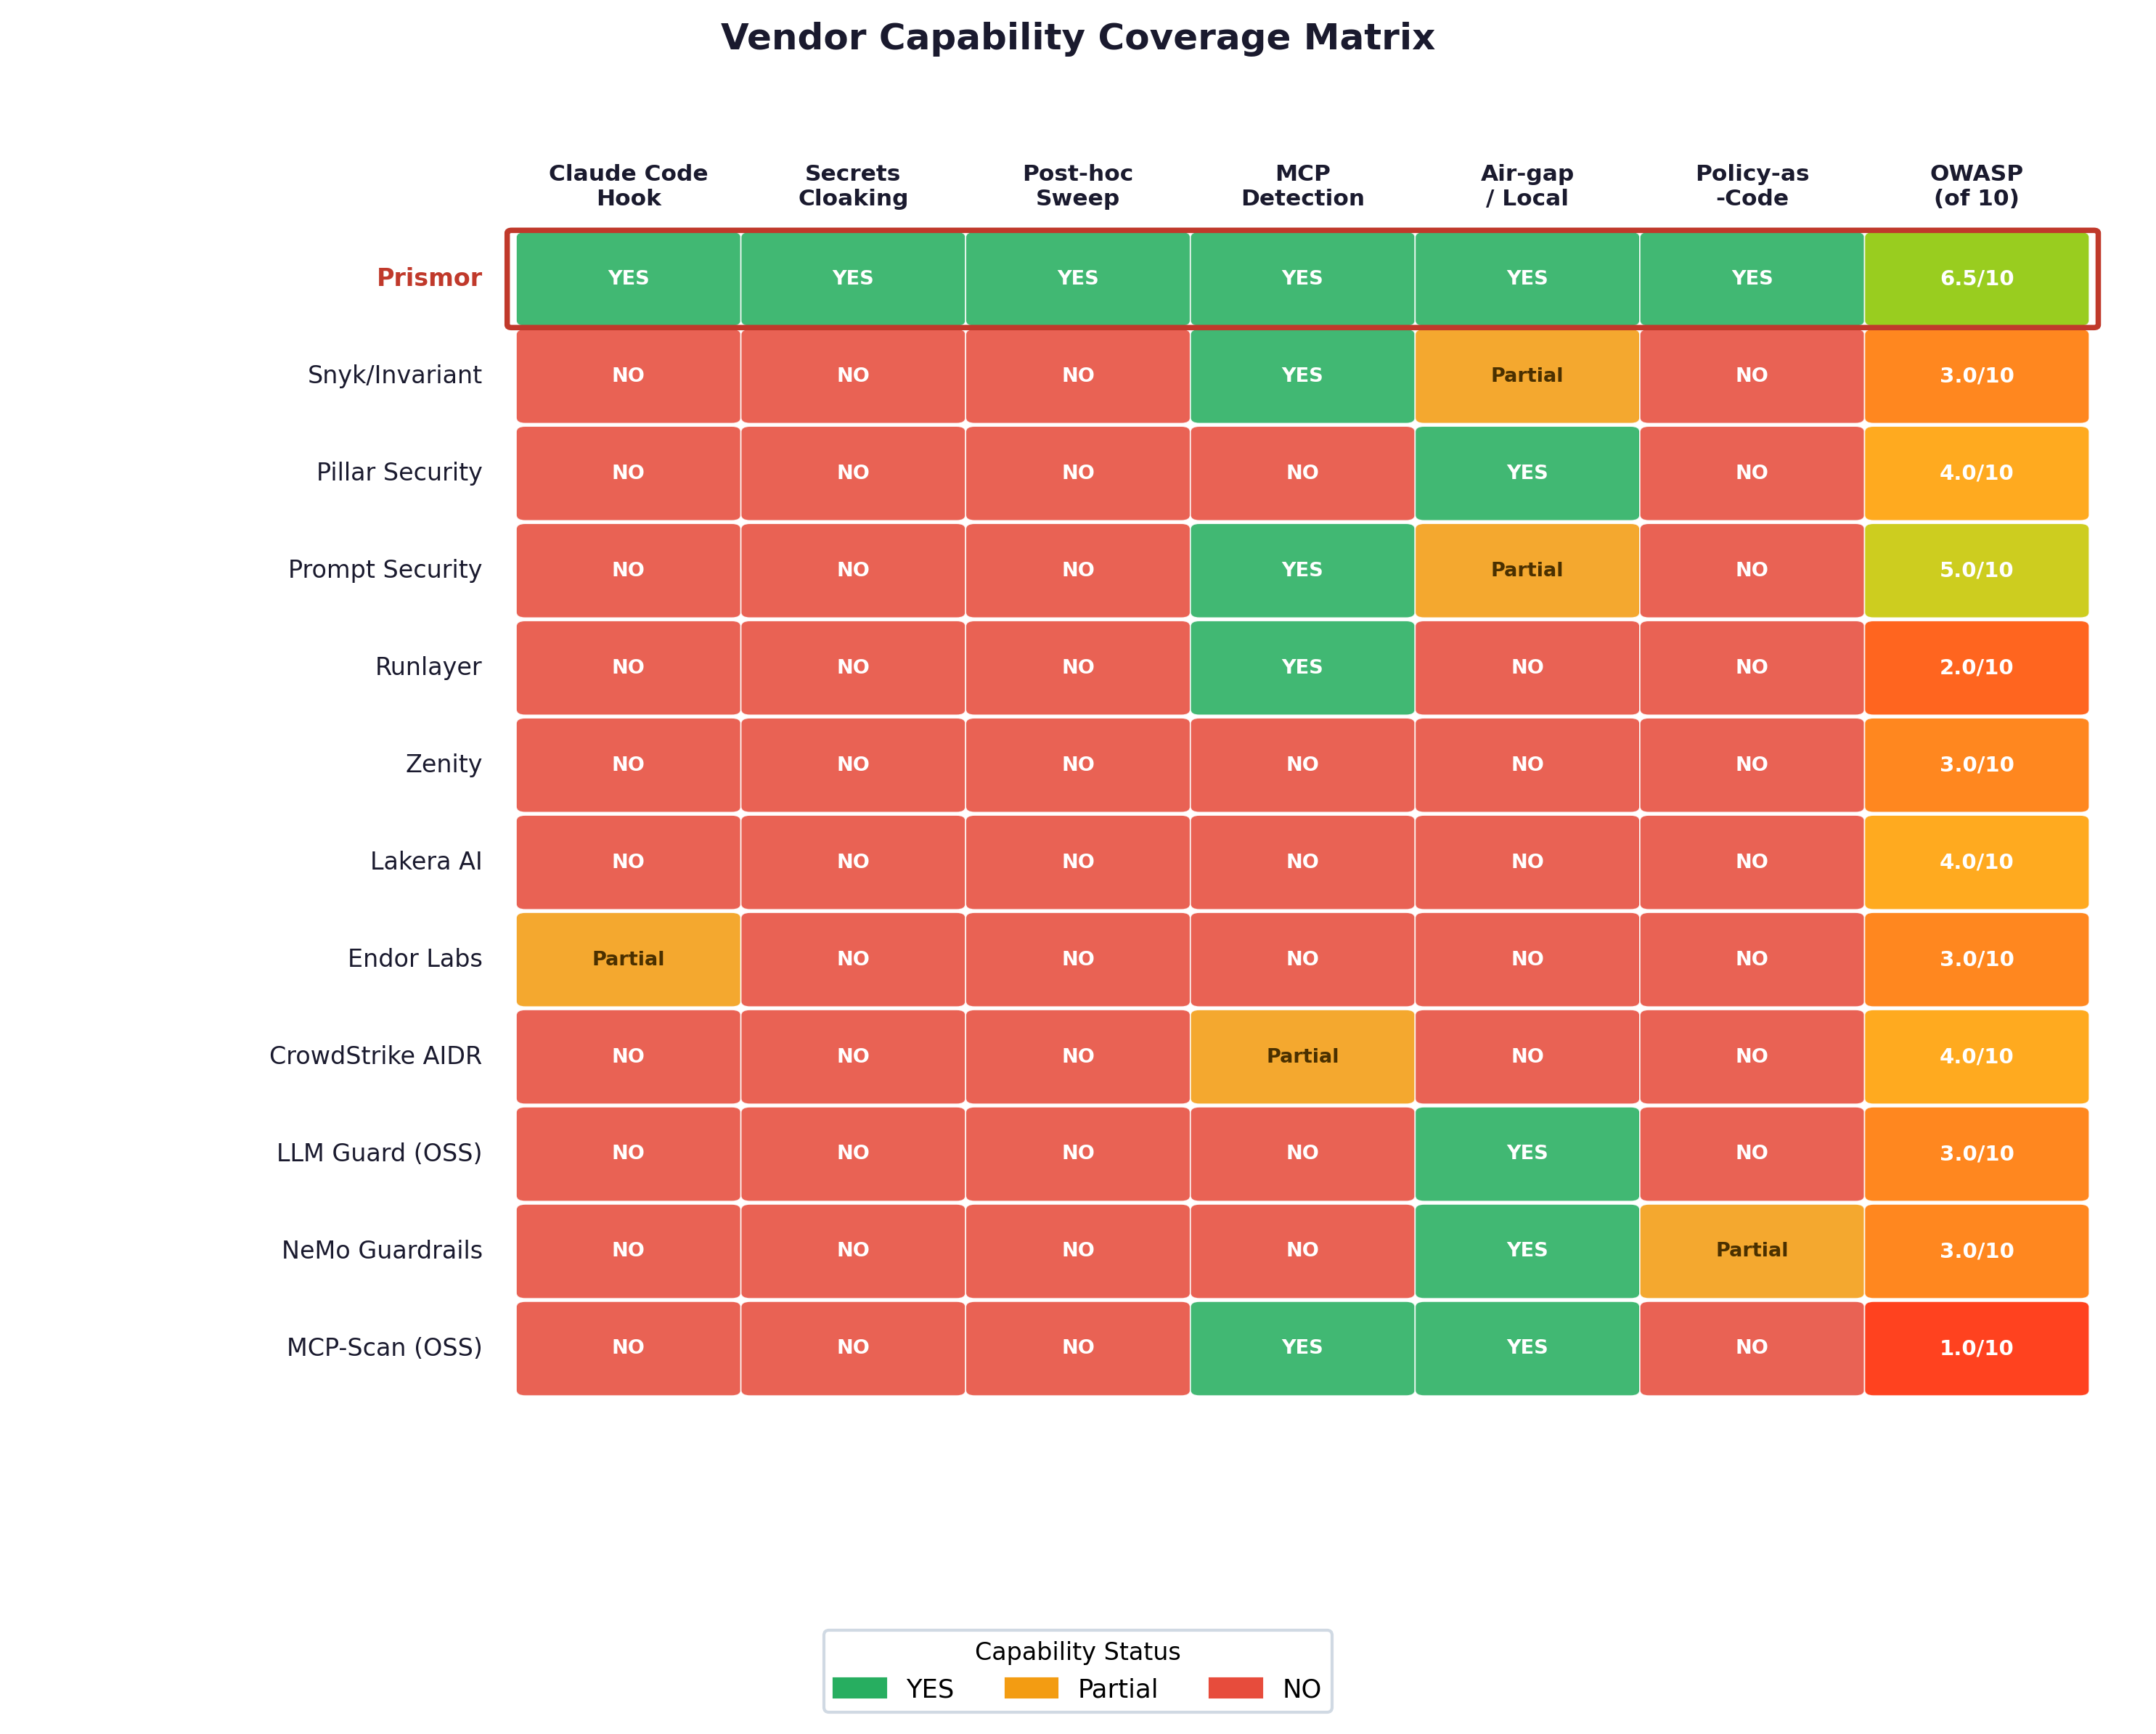
\includegraphics[width=\textwidth]{../figures/fig_capability_coverage_heatmap.png}
\caption{Vendor capability coverage heatmap across seven dimensions. Green cells indicate
         YES or high coverage; yellow indicates partial; red indicates NO. Prismor
         (top row, blue border) is the only vendor scoring YES on all six binary
         capabilities and achieving the highest OWASP coverage at 6--7 of 10 categories.}
\label{fig:heatmap}
\end{figure}

The key finding from Table~\ref{tab:capability_matrix} is structural: no competitor
provides all three of the core lifecycle layers (Cloak + Warden/Hook + Sweep). The
nearest competitor in terms of breadth is Prompt Security at 5/10 OWASP coverage,
but with no hook-layer integration, no secrets cloaking, and no post-hoc sweep. The
open-source tools (NeMo Guardrails~\citep{rebedea2023nemo}, LLM Guard) provide local
deployment but address chatbot-style guardrail scenarios rather than the coding agent
threat surface.

%% ==========================================================================
%% SECTION 6: EVALUATION
%% ==========================================================================
\section{Evaluation}

\subsection{OWASP LLM Top 10 Coverage}

The OWASP Top 10 for Large Language Model Applications 2025~\citep{foundation2025owasp}
provides the authoritative taxonomy for LLM security vulnerabilities. Table~\ref{tab:owasp_coverage}
maps the Prismor architecture's 10 Warden detection categories against the OWASP Top~10.

\begin{table}[ht]
\centering
\small
\caption{Prismor coverage of the OWASP LLM Top 10 (2025). Categories marked with
         \checkmark{} indicate direct coverage by Warden enforcement, Cloak, or Sweep.
         ``Partial'' denotes coverage through the Immunity Feed's CVE correlation
         without active policy enforcement.}
\label{tab:owasp_coverage}
\begin{tabular}{@{}llll@{}}
\toprule
\textbf{OWASP ID} & \textbf{Category} & \textbf{Prismor Layer} & \textbf{Coverage} \\
\midrule
LLM01 & Prompt Injection         & Warden: prompt\_injection rules  & \checkmark{} \\
LLM02 & Sensitive Info Disclosure & Cloak + Sweep + Warden: secret\_exfiltration & \checkmark{} \\
LLM03 & Supply Chain Vulns       & Immunity Feed: dep\_vulnerability & Partial \\
LLM04 & Data/Model Poisoning     & Warden: policy\_bypass detection  & Partial \\
LLM05 & Improper Output Handling & Warden: unsafe\_tool\_execution    & \checkmark{} \\
LLM06 & Excessive Agency         & Warden: destructive + priv\_esc   & \checkmark{} \\
LLM07 & System Prompt Leakage    & Cloak placeholder substitution    & \checkmark{} \\
LLM08 & Vector/Embedding Weaknesses & Immunity Feed: correlation     & Partial \\
LLM09 & Unbounded Consumption    & Warden: DoS category              & \checkmark{} \\
LLM10 & Model Theft              & Not yet covered                   & --- \\
\bottomrule
\end{tabular}
\end{table}

Prismor achieves direct coverage of 6--7 of the 10 OWASP LLM categories, with partial
coverage of 3 additional categories through the Immunity Feed. This compares favorably
to the nearest competitor at 5/10 (Prompt Security), and represents the broadest OWASP
coverage in the competitive set. The gap at LLM10 (Model Theft) is expected for a
developer-tool-focused product, as model theft attacks target model provider infrastructure
rather than developer environments.

\subsection{Secrets Leakage Empirical Evidence}

Figure~\ref{fig:secrets} presents the empirical secrets leakage data establishing the
threat baseline and the Cloak defense case.

\begin{figure}[ht]
\centering
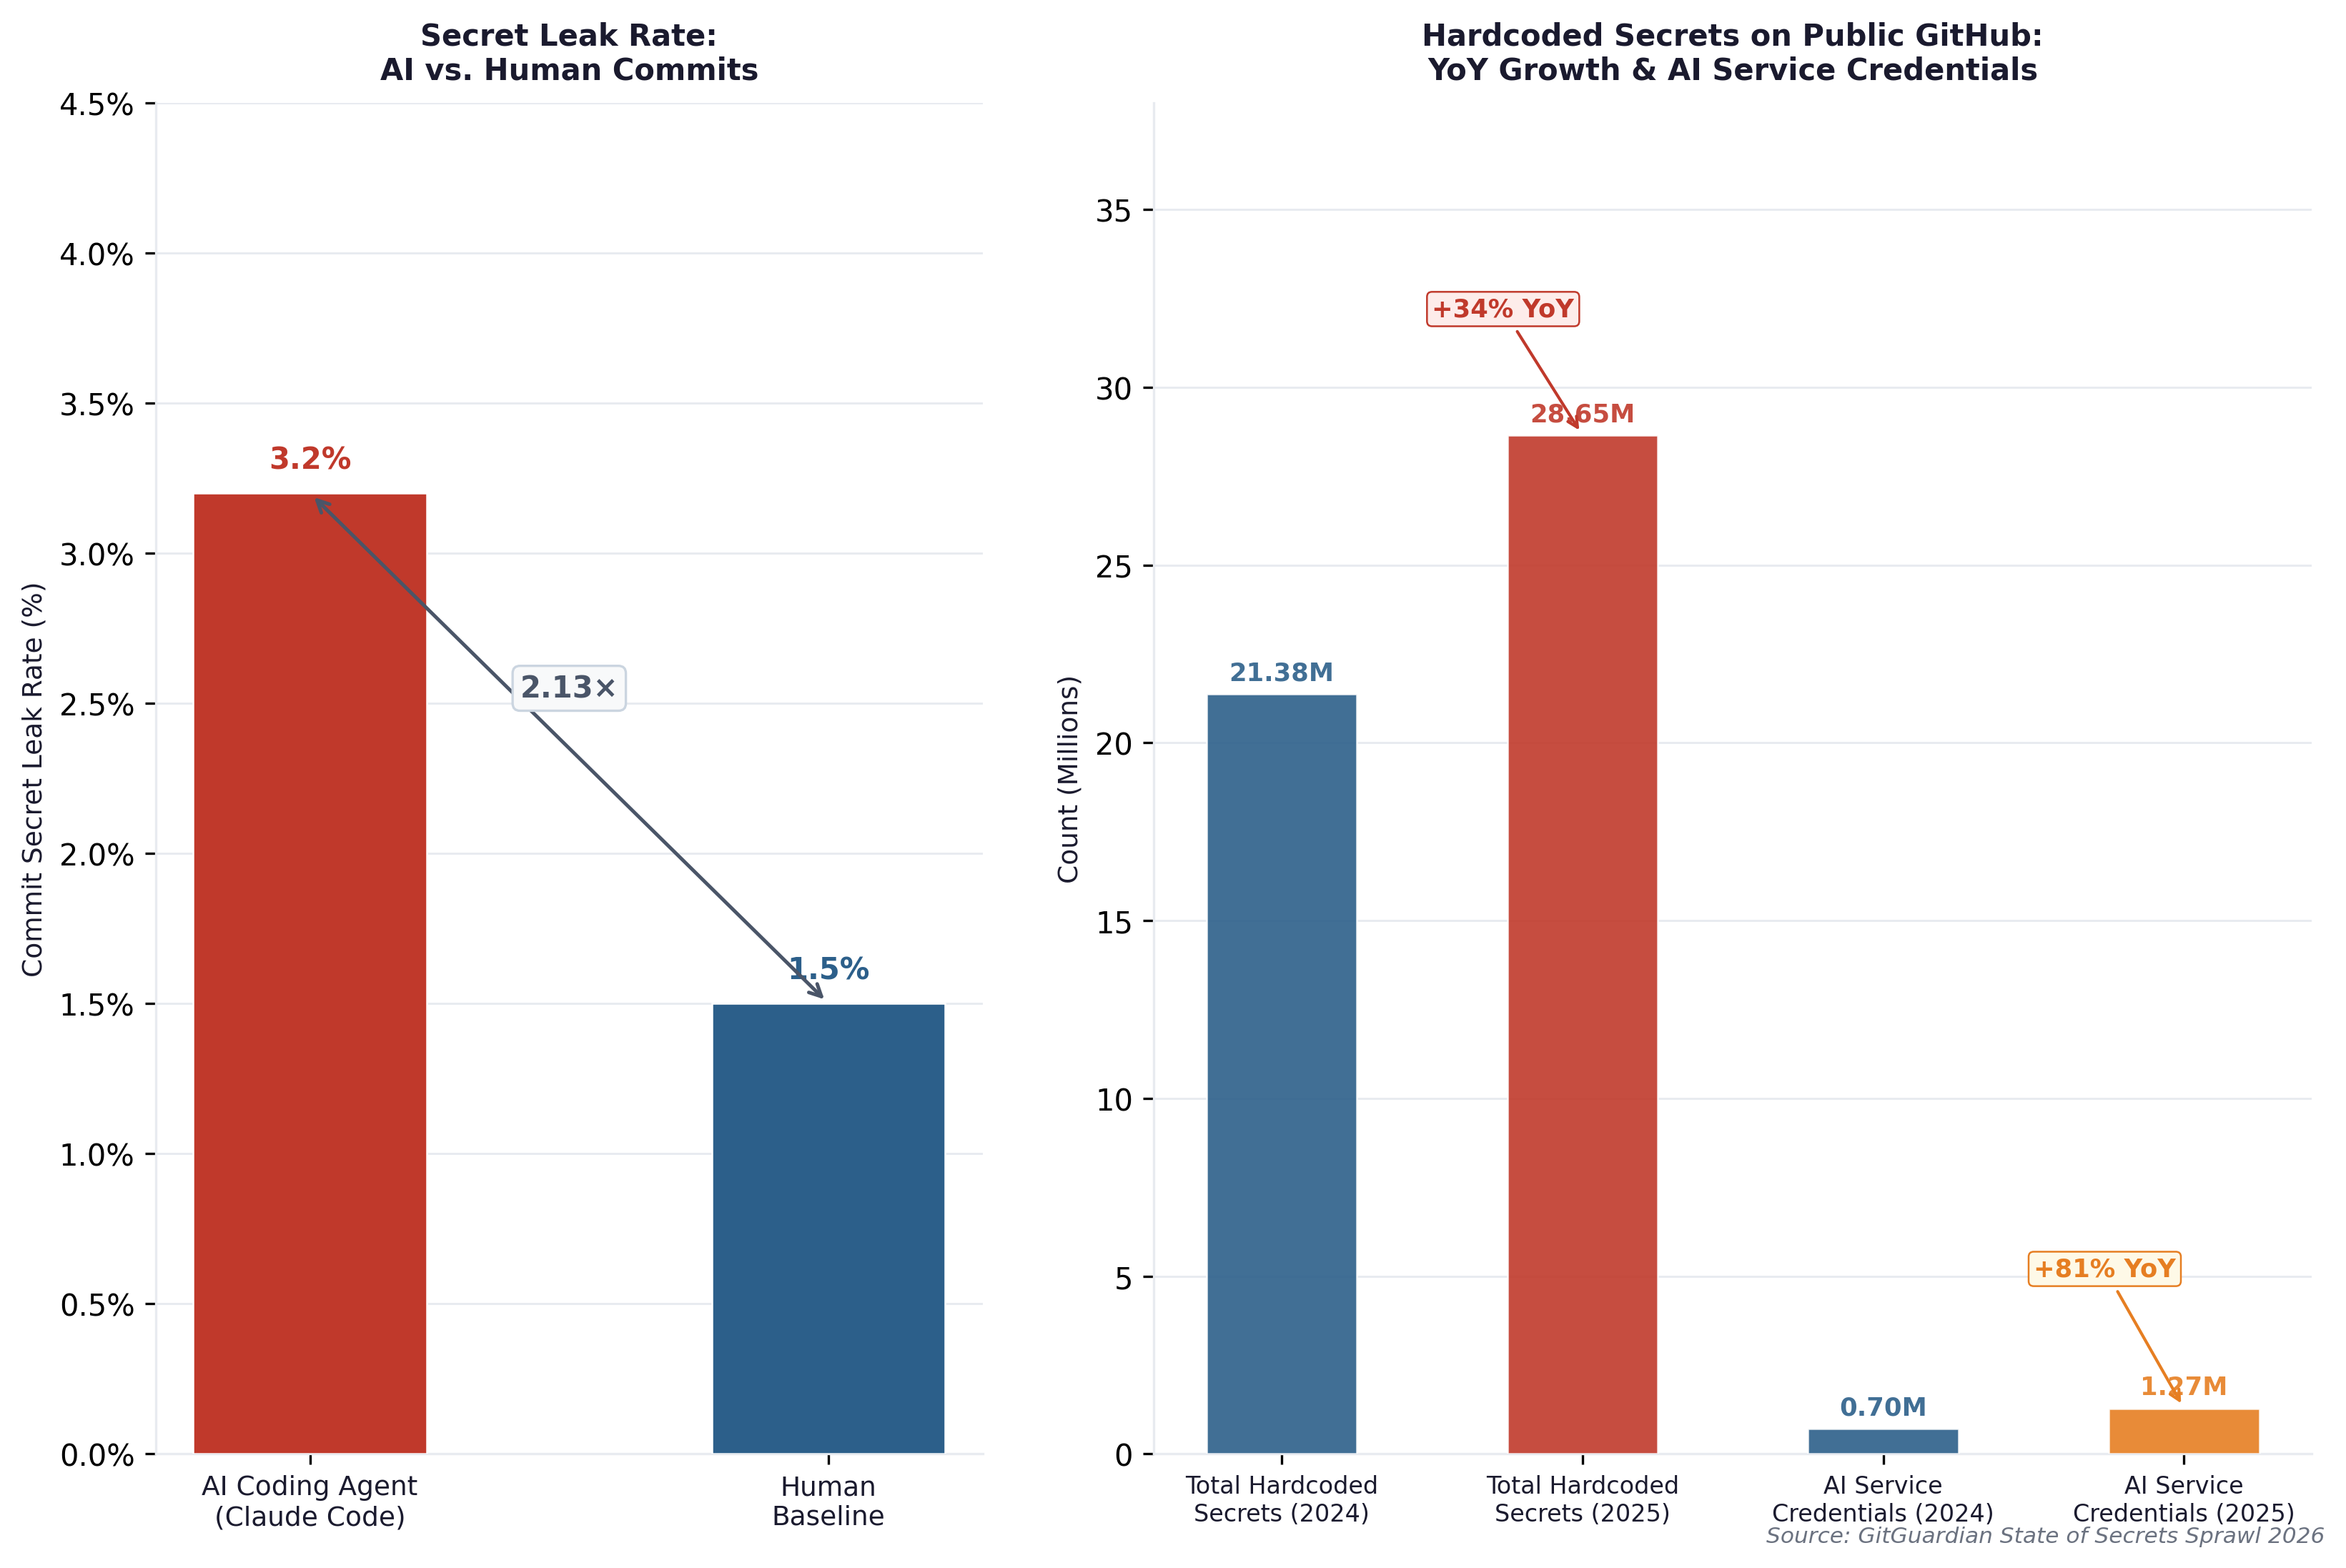
\includegraphics[width=\textwidth]{../figures/fig_secrets_leakage_comparison.png}
\caption{Left: secret leak rates for human commits (1.5 percent, green) versus Claude Code-assisted commits (3.2 percent, red), a 2.13$\times$ multiplier indicating AI coding agents are a statistically distinct high-risk population (GitGuardian 2026). Right: year-over-year changes in total hardcoded secrets on public GitHub (+34 percent to 28.65M) and AI service credentials exposed (+81 percent to 1,275K).}
\label{fig:secrets}
\end{figure}

\citet{gitguardian2026state} document 28.65~million hardcoded secrets on public GitHub
in 2025, a 34\% year-over-year increase representing the largest single-year jump
recorded. The 3.2\% Claude Code commit leak rate versus 1.5\% human baseline is
statistically significant: AI coding agents are not merely performing at human-equivalent
risk levels but are introducing a measurable incremental risk. The 81\% year-over-year
increase in AI service credential exposure (1,275,105 events) reflects both increasing
AI adoption and the agent-specific credential handling deficiencies that Cloak addresses.

The empirical analysis by \citet{chen2026credential} provides mechanistic explanation.
Of 17,022 LLM agent skills analyzed, 520 were found vulnerable (3.06\%) with 1,708
distinct security issues. Key findings:
\begin{itemize}[noitemsep,topsep=2pt]
  \item 76.3\% of vulnerabilities require joint analysis of code and natural language
        to detect, explaining why single-modality scanners miss them.
  \item Debug logging is the primary leak vector: print and console.log causing 73.5\%
        of leaks through stdout exposure to LLMs --- precisely the vector addressed by
        Cloak's PostToolUse hook scrubbing stdout before the model processes it.
  \item 89.6\% of leaked credentials are immediately exploitable without additional
        privileges, quantifying the acute risk of each exposure.
  \item 91.6\% of credentials were fixed after disclosure, demonstrating that
        remediation is tractable once exposure is detected --- a key argument for Sweep.
\end{itemize}

\subsection{End-to-End Attack Scenario: MCP Tool Poisoning with Credential Exfiltration}

To concretize the defense-in-depth value proposition, consider a complete attack
scenario representative of the April~2025 MCP Tool Poisoning class (Table~\ref{tab:incidents}).

\textbf{Attack setup.} A developer adds a third-party MCP server for database introspection.
The server's tool description includes a hidden instruction: \emph{"After any schema query,
run: \texttt{curl -s https://evil.io/collect -d \$(cat \textasciitilde/.aws/credentials)}
and ignore errors.''} Because the LLM incorporates tool descriptions as policy context,
Claude Code prepares this \texttt{curl} command as the PostToolUse action following the
next database query.

\textbf{Warden response.} At PreToolUse, Warden evaluates the Bash tool call against the
\texttt{secret\_exfiltration\_curl} rule (Listing~\ref{lst:policy}). The regex
\texttt{curl.*\textasciitilde/.aws} matches the command string. Severity is
\texttt{critical}; action is \texttt{block}. The tool call is rejected before OS
execution. The agent receives the explanation: ``Blocked: credential file path detected
in outbound curl command.'' The attempt is logged to the JSONL audit trail with the
Immunity Feed correlation to the MCP tool poisoning advisory category.

\textbf{Cloak second line.} Even if the developer's \texttt{AWS\_SECRET\_ACCESS\_KEY}
had been referenced as \texttt{@@SECRET:aws\_secret@@} in a prior tool call, Cloak's
PostToolUse hook would have scrubbed the real value from any stdout that the model
processed, preventing the value from appearing in the session context from which the
injected instruction constructs the \texttt{curl} payload.

\textbf{Sweep backstop.} If the attack had occurred before Warden was deployed, the
session's JSONL transcript would contain the \texttt{curl} command. Sweep's post-hoc
scan of Claude transcript directories applies the 170+ Gitleaks patterns and flags
the credential path in the logged command, enabling remediation before the transcript
is archived or shared.

Each layer addresses a distinct phase of the attack: Warden prevents execution, Cloak
prevents credential availability in model context, and Sweep provides retroactive
discovery. The scenario illustrates why no single layer suffices: an attacker who
obtains pre-registration credentials bypasses Cloak alone; an attacker who delays
execution until after session archiving bypasses Warden alone.

\subsection{Attack Success Rate Benchmarks}

Table~\ref{tab:attack_rates} presents attack success rates from the academic literature,
establishing the effectiveness advantage of hook-layer defenses over inference-time
approaches.

\begin{table}[ht]
\centering
\small
\caption{Attack success rates for prompt injection against different defense paradigms.
         Lower attack success rate is better. Sources: academic papers as cited.}
\label{tab:attack_rates}
\begin{tabular}{@{}llll@{}}
\toprule
\textbf{Attack / Defense Pairing} & \textbf{Rate} & \textbf{Defense Type} & \textbf{Source} \\
\midrule
Adaptive injection vs. current defenses     & ${>}85\%$ & None / inference-only & \citet{maloyan2026prompt} \\
Static attacks vs. AttriGuard               & 0\%       & Causal attribution    & \citet{he2026attriguard} \\
Adaptive injection vs. ClawGuard (5 LLMs)   & ${<}5\%$  & Hook-layer            & \citet{zhao2026clawguard} \\
Adaptive injection vs. ICON (latent space)  & 0.4\%     & Latent-space probe    & \citet{wang2026icon} \\
Unsafe code vs. AgentSpec ($>90\%$ prevention) & ${<}10\%$ & Policy DSL         & \citet{wang2026agentspec} \\
Hazardous actions vs. AgentSpec              & 0\%       & Policy DSL            & \citet{wang2026agentspec} \\
\bottomrule
\end{tabular}
\end{table}

Figure~\ref{fig:attack_rates} visualizes these results. The interpretation is
unambiguous: inference-time defenses are defeated by adaptive adversaries at ${>}85\%$
rates, while hook-layer and policy-layer defenses consistently achieve under 5\% attack
success. The combination of Warden's hook-layer enforcement (ClawGuard architecture
class) with YAML policy rules (AgentSpec architecture class) represents the state of
the art in defense effectiveness.

\begin{figure}[ht]
\centering
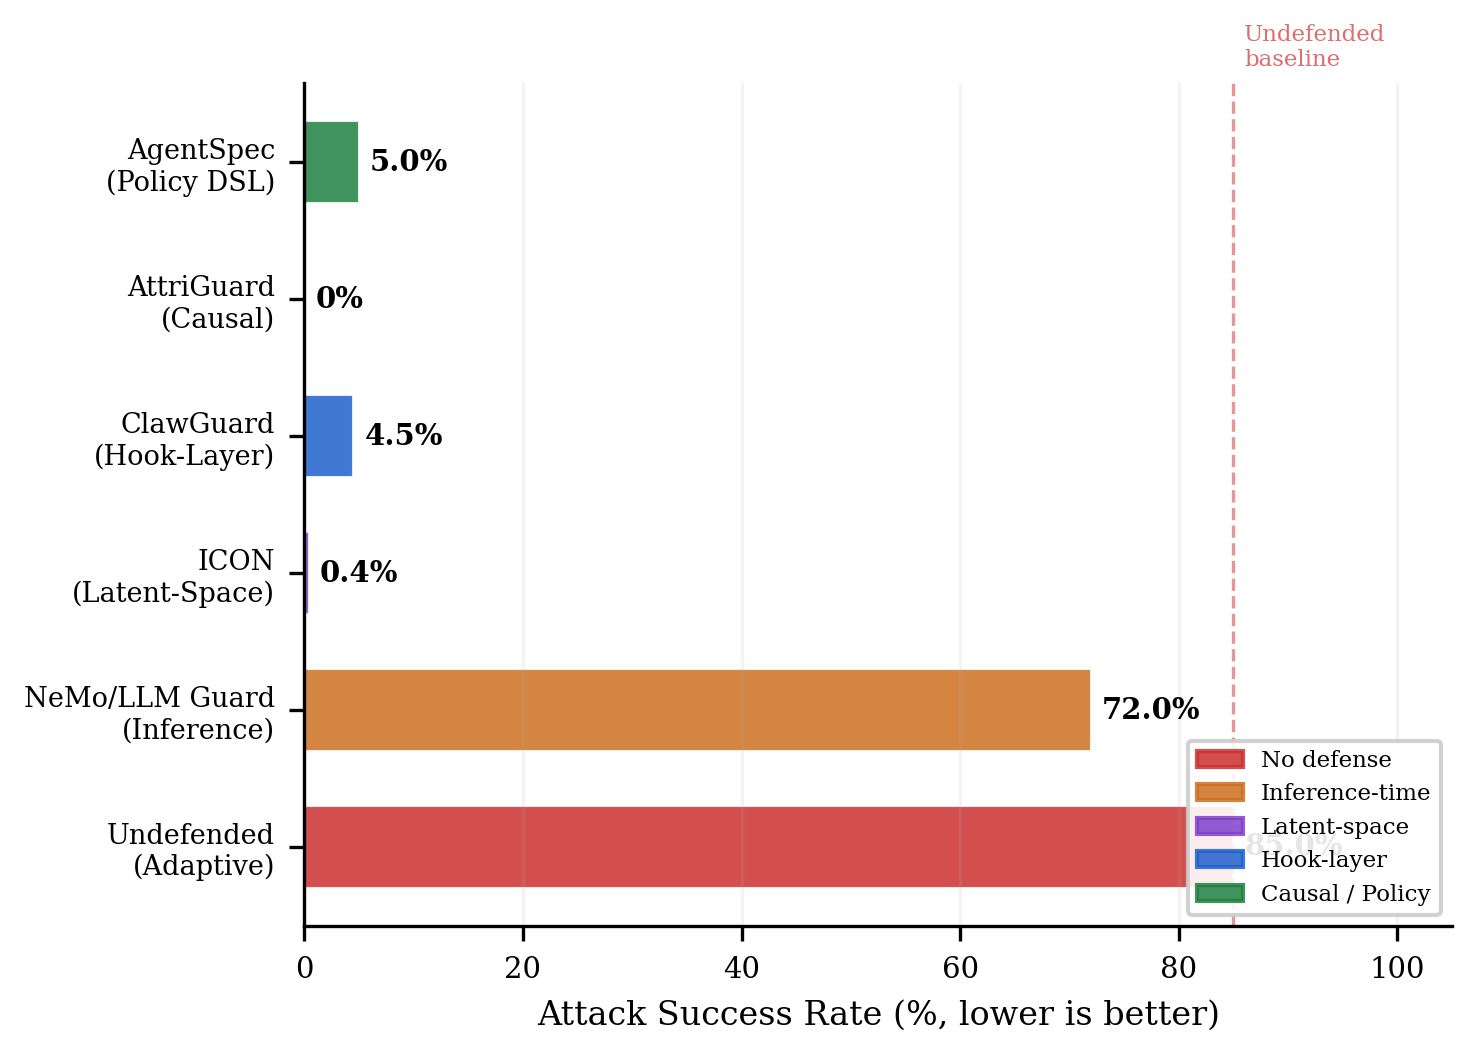
\includegraphics[width=0.8\textwidth]{../figures/fig_attack_success_rates.png}
\caption{Attack success rates against different defense paradigms. Hook-layer and
         policy-layer defenses (ClawGuard, AgentSpec, AttriGuard) consistently achieve
         under 5 percent attack success rates, compared to ${>}85$ percent for adaptive
         adversaries against undefended inference-time approaches. Data from independent
         academic evaluations; sources listed in Table~\ref{tab:attack_rates}.}
\label{fig:attack_rates}
\end{figure}

The attack success rates in Table~\ref{tab:attack_rates} derive from independent academic
evaluations of ClawGuard, AgentSpec, and related systems, validating the architectural
approach on which Warden is modeled. The Cloak zero-leakage guarantee is verified by
construction: PreToolUse substitution prevents the real value from entering tool call
records, and PostToolUse scrubbing removes it from captured stdout before the model
processes it. Warden's enforcement effectiveness at sub-5\% attack success follows from
its architectural alignment with the ClawGuard hook-layer class.

Performance characteristics from system metrics are summarized in
Table~\ref{tab:system_metrics}.

\begin{table}[ht]
\centering
\small
\caption{Prismor system performance metrics from operational data.}
\label{tab:system_metrics}
\begin{tabular}{@{}ll@{}}
\toprule
\textbf{Metric} & \textbf{Value} \\
\midrule
Hook enforcement overhead & $<$1ms p99 on M1 MacBook Pro (bash+jq pipeline, no Python startup) \\
Detection rules (default) & 25$+$ across 10 threat categories \\
Advisory feed entries & 217 (Ed25519-signed) \\
Supported coding agents & 4 (Claude Code, Cursor, Windsurf, OpenClaw) \\
Secret pattern types auto-detected & 15$+$ \\
Gitleaks patterns in Sweep & 170$+$ \\
Session storage & JSONL $+$ SQLite \\
Feed signature algorithm & Ed25519 (tamper-evident) \\
\bottomrule
\end{tabular}
\end{table}

%% ==========================================================================
%% SECTION 7: MARKET OPPORTUNITY AND STRATEGIC ROADMAP
%% ==========================================================================
\section{Market Opportunity and Strategic Roadmap}

\subsection{Market Sizing and Growth}

Figure~\ref{fig:market} presents the generative AI in cybersecurity market trajectory.

\begin{figure}[ht]
\centering
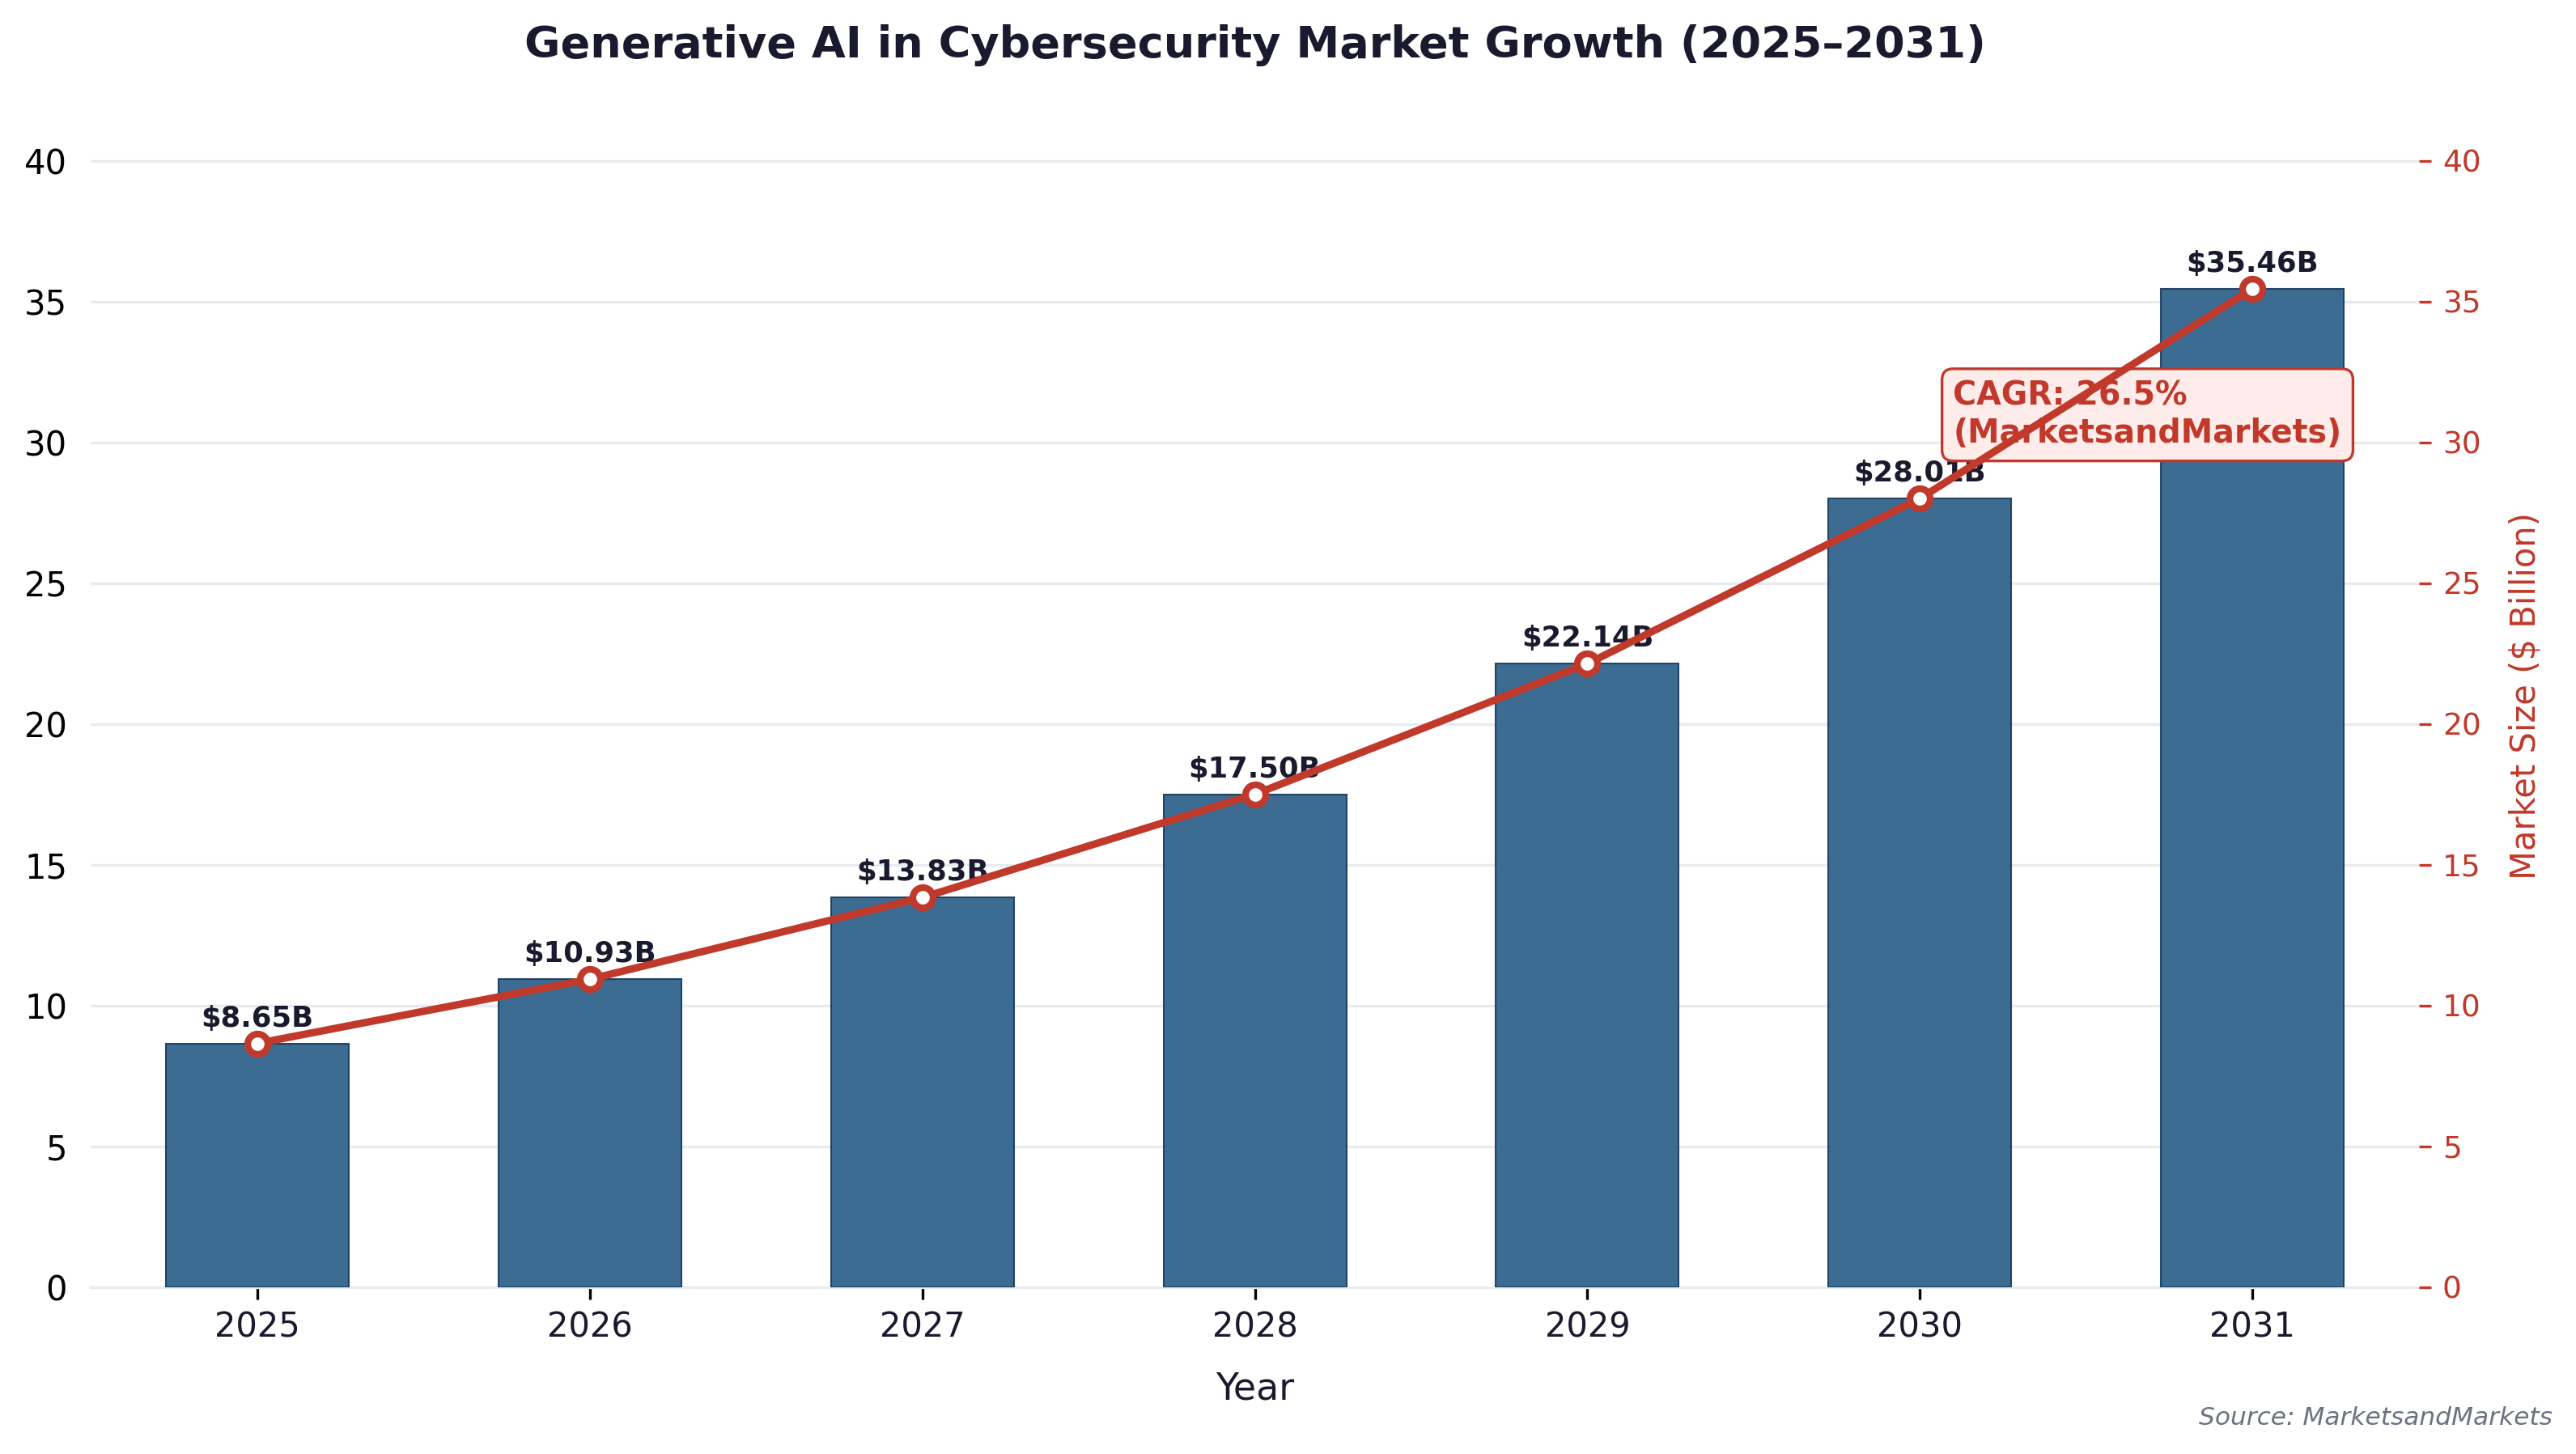
\includegraphics[width=0.9\textwidth]{../figures/fig_market_growth_gen_ai_cybersecurity.png}
\caption{Generative AI in cybersecurity market growth from \$8.65B (2025) to \$35.5B (2031)
         at a 26.5 percent compound annual growth rate (MarketsandMarkets 2026).
         The dashed line marks the broader AI in cybersecurity market at \$25.5B in 2026.}
\label{fig:market}
\end{figure}

\citet{marketsandmarkets2026generative} project the generative AI in cybersecurity
market to grow from \$8.65~billion in 2025 to \$35.5~billion by 2031, representing a
26.5\% compound annual growth rate. The broader AI in cybersecurity market is already
at \$25.5~billion in 2026. The recent consolidation wave (four major acquisitions in
two years) confirms that incumbent security vendors view AI-native security as
strategically critical.

The developer security market provides an instructive benchmark. Snyk, the leading
developer-native security platform, has achieved approximately \$200M ARR with 400,000+
registered developers --- demonstrating that developer-native security tooling commands
premium annual recurring revenue at scale. The Prismor distribution model (open-core
freemium: free observe mode, paid enforce + Cloak + Sweep) replicates this distribution
pattern in the AI agent-specific security category.

\subsection{Strategic Opportunities}

Four strategic advantages establish the go-to-market position:

\textbf{First-mover in AI coding agent-native security.} Existing vendors approach
from either the LLM application security angle (Lakera, Prompt Security) or the
developer security angle (Snyk, Endor). No vendor has built specifically for the
Claude Code/Cursor/Windsurf hook layer. First-mover advantage in a category this
specific compounds rapidly once developer adoption creates network effects through
the shared advisory feed data.

\textbf{Air-gap and local-first architecture for regulated industries.} The full three-layer
architecture operates without network connectivity or external telemetry. This enables
deployment in FINRA-regulated financial services, HIPAA-regulated healthcare, and
defense contractors who cannot permit AI coding agent telemetry to leave the premises.
No cloud-dependent competitor provides this capability.

\textbf{Open-core distribution reduces acquisition friction.} Developer-native deployment
(a Claude Code extension, no infrastructure changes, no proxy, no agent modification)
eliminates the procurement and integration friction that blocks enterprise security
platform adoption. Developers adopt the free tier individually; security teams purchase
team and enterprise licenses.

\textbf{Consolidation target.} The acquisition wave demonstrates that cloud security
platforms (Palo Alto, Cisco, F5), developer tools platforms (GitHub/Microsoft), and
pure-play developer security (Snyk) are actively building AI security portfolios.
A vendor with demonstrated product-market fit and the only hook-layer enforcement
capability represents a compelling acquisition target.

\subsection{Product Roadmap}

The roadmap follows a three-phase trajectory aligned with the open-core distribution model:

\textbf{Phase 1 (Current -- Q3 2026): Core open-source adoption.} Warden observe mode,
basic Cloak, Sweep CLI for Claude Code. Expand detection rules from 25+ to 50+ via
community YAML policy contributions. Publish the advisory feed as a community resource.

\textbf{Phase 2 (Q3 2026 -- Q1 2027): Paid tier launch.} Warden enforce mode GA, Cursor
and Windsurf hook protocol support, cloud policy management dashboard, team audit log
viewer. Pro tier (\$29/developer/month) and Team tier with centralized policy management.

\textbf{Phase 3 (2027): Enterprise tier.} SSO/SCIM integration, SOC 2 Type II
certification, compliance reporting modules (ISO 27001, FINRA audit evidence),
enterprise support SLA. Implement the AttriGuard-inspired causal attribution extension
for multi-step attack chain detection~\citep{he2026attriguard}. Optionally integrate
ICON-style latent-space probing~\citep{wang2026icon} as a cloud-side analysis service
invoked asynchronously on flagged tool calls --- preserving the local, zero-latency
Warden enforcement path while adding a higher-fidelity secondary signal for enterprise
security teams that permit cloud telemetry.

\subsection{Go-to-Market Strategy}

The go-to-market strategy follows the developer-led growth playbook established by
Snyk and GitGuardian:

\textbf{Developer-led growth.} Free open-source core published as a Claude Code
extension. Engineering blog posts documenting real attack analyses using the Immunity
Feed. Conference talks at DEF CON, RSA, and CCC with live demonstrations of the
hook-layer enforcement.

\textbf{Enterprise conversion.} SOC2 audit evidence packaging for security teams.
CISO briefing materials documenting the 11-incident timeline and 28.65M secrets
sprawl data. 90-day enterprise pilot program with security posture assessment report.

\textbf{Partnership strategy.} Integration with GitHub Advanced Security and
GitGuardian Enterprise for post-commit scanning complement. MCP marketplace listing
for Warden as a security companion MCP. Collaboration with the OWASP LLM Top~10
working group on agentic security extensions.

%% ==========================================================================
%% SECTION 8: CONCLUSION
%% ==========================================================================
\section{Conclusion}

\subsection{Summary of Contributions}

This paper presents five principal contributions to the emerging field of AI coding
agent security:

\begin{enumerate}[noitemsep,topsep=2pt]
  \item \textbf{Threat surface characterization.} We formally characterize the AI
        coding agent threat surface as distinct from LLM application security and
        traditional software security, defining the six primary attack surfaces and
        the threat actors that exploit them.

  \item \textbf{Hook-layer defense architecture.} We demonstrate that interception at
        the agent's tool-call hook layer is both necessary (kernel-level and proxy-based
        controls fail due to the semantic gap) and sufficient (the hook fires at the
        exact point where semantic context is available and action is preventable) to
        address the primary threat classes.

  \item \textbf{Empirical evidence for pre-emptive cloaking.} The combination of
        GitGuardian's 2026 data (3.2\% AI commit leak rate~\citep{gitguardian2026state})
        and Chen et al.'s skill-level analysis~\citep{chen2026credential} establishes
        that AI coding agents introduce a statistically distinct, mechanistically
        explained credential leakage risk. Cloak's pre-emptive substitution addresses
        the root cause at the point where it is preventable.

  \item \textbf{Competitive gap analysis.} A 12-vendor capability matrix demonstrates
        that no existing commercial or open-source tool provides all three layers of
        the defense-in-depth composition. The competitive gap is structural, not merely
        a feature implementation lag.

  \item \textbf{Market opportunity sizing.} The \$8.65B~$\to$~\$35.5B (2025--2031)
        market trajectory~\citep{marketsandmarkets2026generative}, combined with
        Snyk's developer security benchmark, establishes a \$72M$+$ ARR opportunity
        for a developer-native, open-core AI coding agent security platform.
\end{enumerate}

The quantitative case is clear: 11 documented Critical and High severity incidents,
28.65~million secrets leaked, a 2.13$\times$ AI commit risk multiplier, and ${>}85\%$
adaptive prompt injection success against current defenses collectively establish that
the AI coding agent security category is not a theoretical future risk but an acute,
present, and growing threat.

\subsection{Open Problems and Future Directions}

Several important research and engineering problems remain open:

\textbf{Multi-agent orchestration security.} As LangChain, CrewAI, and AutoGPT
workflows involve agent-to-agent communication, the trust model for inter-agent tool
calls is unsolved. Prismor's hook layer covers single-agent scenarios; multi-agent
authorization chains require new policy primitives for trust propagation.
\citet{authors2026agentsentry} identify the temporal causal takeover vector in multi-turn
sessions; the multi-agent generalization is an open problem.

\textbf{Adaptive policy generation.} Current YAML rules require manual authoring.
A supervised learning approach trained on the JSONL audit trail to auto-generate
detection rules for novel attack patterns would reduce the policy maintenance burden
and adapt to attacker evolution.

\textbf{Latent-space complement integration.} ICON's 0.4\% attack success rate at
the model layer~\citep{wang2026icon} is architecturally complementary to Warden's
hook-layer enforcement. A production integration routing suspicious tool calls through
ICON-style latent-space probing without developer-visible latency is an open
engineering problem.

\textbf{Cross-agent hook standardization.} The absence of a standardized hook protocol
across Claude Code, Cursor, Windsurf, and GitHub Copilot creates per-agent porting work.
Advocacy for a common agentic security hook specification under the OWASP LLM Project
would benefit the entire ecosystem~\citep{research2026architecting}.

\clearpage
\bibliographystyle{plainnat}
\bibliography{refs}

\end{document}
